\documentclass[a4paper,10pt,titlepage,oneside,openany]{book}

% ===== Pacchetti =====
\usepackage[skip=6pt]{parskip}
\usepackage[english]{babel}
\usepackage[utf8]{inputenc}
\usepackage[T1]{fontenc}
\usepackage{graphicx}
\usepackage{amsmath,amssymb}
\usepackage{amsthm}
\usepackage{enumitem}
\usepackage{float}
\usepackage{changepage} % per adjustwidth in pseudocode
\usepackage[top=1in, bottom=1in, left=1in, right=1in]{geometry}
\usepackage{fancyhdr}
\usepackage{tcolorbox}
\usepackage{array}
\usepackage{booktabs}
\usepackage{tabularx}
\usepackage{pdfpages}
\usepackage[colorlinks=true, linkcolor=black, citecolor=black, urlcolor=blue]{hyperref}
\usepackage{etoolbox}   % patch capitoli
\usepackage{ragged2e}   % per \justifying

% Pacchetti aggiuntivi necessari al corpo del paper
\usepackage{mathtools}
\usepackage{caption}
\usepackage{subcaption}
\usepackage[ruled,vlined]{algorithm2e}
\usepackage{listings}
\usepackage{xcolor}

% Compatibilita' con citazioni in stile \textcite senza biblatex
\providecommand{\textcite}[1]{\cite{#1}}

% Giustificazione e no-indent di default su tutto il documento
\AtBeginDocument{\justifying}
\setlength{\parindent}{0pt}
\setlength{\parskip}{6pt}

% -------------------------------
% Da cambiare quando si copia il template in \graphicspath{{img/}{1/}}
% -------------------------------
\graphicspath{{img/}{1/}}

% ===== Header / Footer =====
\pagestyle{fancy}
\fancyhf{}
\fancyhead[L]{\textbf{Starting Finance Club PoliTo}}
\fancyhead[R]{
\includegraphics[width=1cm]{img/Logo_SFClub_Polito.png}}
\fancyfoot[C]{\thepage}
\renewcommand{\headrulewidth}{0.4pt}
\renewcommand{\footrulewidth}{0.4pt}
\setlength{\headheight}{33pt}
\setlength{\headsep}{24pt} % spazio sotto l'header

\fancypagestyle{plain}{%
  \fancyhf{}
  \fancyhead[L]{\textbf{Starting Finance Club PoliTo}}
  \fancyhead[R]{
\includegraphics[width=1cm]{img/Logo_SFClub_Polito.png}}
  \fancyfoot[C]{\thepage}
  \renewcommand{\headrulewidth}{0.4pt}
  \renewcommand{\footrulewidth}{0.4pt}
}

% ===== Ambienti theorem ecc. =====
\theoremstyle{plain}\newtheorem{theorem}{Theorem}[chapter]
\theoremstyle{definition}\newtheorem{definition}{Definition}[chapter]
\newtheorem{notation}{Notation}[chapter]
\theoremstyle{remark}\newtheorem{remark}{Remark}[chapter]

\newenvironment{pseudocode}{\par\small\ttfamily\begin{adjustwidth}{1em}{1em}}{\end{adjustwidth}\par}

\newenvironment{tightabstract}[1][0.88]{%
  \begin{center}
  \begin{tcolorbox}[title={Abstract}, width=#1\textwidth, left=5mm, right=5mm,
    colback=white, boxrule=0.4pt]
  \small\justifying
}{%
  \end{tcolorbox}
  \end{center}
}

\newenvironment{references}{\begin{thebibliography}{99}}{\end{thebibliography}}

\newcommand{\miniabstract}[1]{%
\vspace{-2pt}
\begin{tcolorbox}[colback=gray!6,colframe=black!15,boxrule=0.3pt,arc=3pt,left=6pt,right=6pt,top=4pt,bottom=4pt]
\textit{Mini-abstract.} #1
\end{tcolorbox}
\vspace{-4pt}
}

% ===== Fix capitoli: -18pt e dimensioni numeriche =====
\makeatletter
\patchcmd{\@makechapterhead}{\vspace*{50\p@}}{\vspace*{-18\p@}}{}{}
\patchcmd{\@makeschapterhead}{\vspace*{50\p@}}{\vspace*{-18\p@}}{}{}
\patchcmd{\@makechapterhead}{\huge}{\fontsize{17}{20}\selectfont\bfseries}{}{}
\patchcmd{\@makechapterhead}{\Huge}{\fontsize{20}{24}\selectfont\bfseries}{}{}
\patchcmd{\@makeschapterhead}{\Huge}{\fontsize{20}{24}\selectfont\bfseries}{}{}
\patchcmd{\@makechapterhead}{\vskip 20\p@}{\vskip 6\p@}{}{}
\patchcmd{\@makechapterhead}{\vskip 40\p@}{\vskip 10\p@}{}{}
\patchcmd{\@makeschapterhead}{\vskip 40\p@}{\vskip 10\p@}{}{}
\makeatother

% ===== Listings =====
\lstdefinestyle{python}{
  language=Python,
  basicstyle=\ttfamily\small,
  keywordstyle=\bfseries,
  commentstyle=\itshape,
  stringstyle=\ttfamily,
  showstringspaces=false,
  breaklines=true,
  frame=single,
  numbers=left,
  numberstyle=\tiny,
  xleftmargin=2em,
  framexleftmargin=1.5em
}
\lstset{style=python}

% ===============================
\begin{document}

% --- Copertina PDF come prima pagina, senza header/footer ---
\includepdf[pages=1,fitpaper=true,pagecommand={\thispagestyle{empty}}]{Copertina_research.pdf}

% --- TITLE/CONTACT/ABSTRACT ---
\begin{titlepage}
\thispagestyle{empty}
\vspace*{-1.5cm}
\begin{center}

\includegraphics[width=3.70cm]{img/Logo_SFClub_Polito.png}\\[1cm]
{\LARGE\bfseries High-Frequency Market Making under Avellaneda--Stoikov\par}
\vspace{0.2cm}
{\large Classical Diffusions and Multi-Asset Inventory Control\par}

\vspace{0.4cm}

% --- Authors + reviewer + date (same size) ---
{\normalsize
\textbf{Authors:}\\[0.3cm]
Salvatore Gabriele Messina\\
Niccol\`o Soriano\\[0.3cm]
\emph{reviewed by}\\[0.15cm]
Michele Gargasole\\[0.4cm]
\textit{Date:} May 15, 2025\par
}

\vspace*{0.1cm}

% --- Only this line in Large (does not affect the rest) ---
{\Large\textbf{Starting Finance Club PoliTo}\par}

\vspace{0.4cm}
\normalsize

\textit{Contact:}\\
\small
LinkedIn: \url{https://www.linkedin.com/company/startingfinance-club-polito}\\
GitHub: \url{https://github.com/StartingFinanceClubPoliTo/Research}\\
Instagram: \url{https://www.instagram.com/sfclubpolito}\\
Website: \url{https://sfclubpolito.it/}

\vspace{1cm}
\begin{tightabstract}
This paper studies high-frequency market making within the Avellaneda--Stoikov framework under classical single-asset price dynamics and a covariance-aware multi-asset extension. It considers two finite-horizon benchmark cases: arithmetic Brownian motion and geometric Brownian motion. Across both cases, it compares a naive symmetric quoting policy with an inventory-based quoting policy derived from the Avellaneda--Stoikov control principle.

The analysis is simulation-first and does not rely on market data. Instead, all experiments are conducted through a unified time-discretized Monte Carlo engine with Poisson fill probabilities that keeps dealer accounting and order-arrival mechanics fixed while varying the mid-price dynamics, and then extends the same logic to vector-valued prices and inventories. The results should therefore be interpreted as a mechanism test under stylized parameters, not as a realistic HFT backtest calibrated to market data. This design isolates the impact of inventory control, multiplicative price risk, and covariance-aware portfolio risk on dealer performance.

The results show how inventory-aware quoting improves risk-adjusted performance by reducing inventory excursions and stabilizing marked-to-market wealth relative to naive quoting. The multivariate extension clarifies how correlated inventories modify quote centers and marginal bid/ask reservation prices. Overall, the study provides a coherent benchmark for understanding the role of classical diffusion modeling and covariance-aware inventory control in high-frequency market making.
\end{tightabstract}
\end{center}
\end{titlepage}

% --- Front matter: TOC in roman numerals starting from i ---
\frontmatter
\clearpage
\pagenumbering{roman}
\setcounter{page}{1} % "i"
\tableofcontents
\thispagestyle{plain}

% --- Main matter: body in arabic ---
\mainmatter
\clearpage
\setcounter{page}{1}

% ===============================
% Body
% ===============================

\chapter*{Introduction and Motivation}
\addcontentsline{toc}{chapter}{Introduction and Motivation}

\section*{Paper Roadmap}
\miniabstract{This introductory section frames the paper's contribution and workflow. Starting from the Avellaneda--Stoikov market making framework, the article uses Monte Carlo simulation to reproduce the canonical qualitative result: relative to a naive symmetric quoting rule, an inventory-based strategy improves risk-adjusted performance by actively controlling inventory exposure, typically reducing the dispersion of terminal wealth and increasing Sharpe-like metrics under comparable experimental conditions. The study is deliberately data-free: rather than calibrating to historical order book data, it adopts stylized parameter regimes and scenario grids in order to isolate mechanisms and ensure transparent reproducibility. Consequently, the numerical results are benchmark diagnostics rather than evidence of deployable HFT profitability. The paper first develops the baseline arithmetic Brownian motion (ABM) mid-price under a finite horizon, then replaces ABM with geometric Brownian motion (GBM) to study non-negative prices and multiplicative fluctuations, and finally rebuilds the model as a covariance-aware multi-asset inventory-control template. This progression isolates how price dynamics and dimensionality affect the naive-versus-inventory-based performance gap.}

\section*{Market making history}
This paper studies the interface between market making and market microstructure through the lens of two time scales. At the daily scale, an asset price can be idealized as a continuous-time process (e.g., a Brownian-motion-like mid-price), and the market maker's problem resembles dynamic risk management with the objective of harvesting the bid--ask spread while controlling inventory exposure. At the sub-second scale, the same environment becomes intrinsically discrete and rule-driven: prices live on a tick grid, orders arrive asynchronously, and the limit order book mechanics and trading frictions shape both the observed price formation and the feasibility of any quoting strategy. The core message is that market making cannot be fully understood at only one resolution: a smooth diffusion view is useful for tractability and control, while a microstructural view is essential for interpreting what the mid-price represents and for implementing strategies under real trading constraints.

Within this perspective, market making can be summarized as an algorithmic decision rule that continuously updates bid and ask quotes as a function of a state vector. Conceptually, the market maker forms a (possibly personal) estimate of value and quotes around it, posting a bid below and an ask above, then adapts these quotes as the state changes, most importantly as the mid-price moves and inventory accumulates. The economic role of this activity is liquidity provision: by standing ready to trade on both sides, the market maker supplies immediacy to other market participants who value execution without delay.

Historically, the intuition of a two-sided quote originated in floor-based settings with designated dealers (often specialists) who were central to trading in a given name. Modern electronic markets replace this institutional structure with competitive, automated quoting in data-center environments, where many agents simultaneously post and cancel orders at high frequency. This evolution motivates the academic progression from classical inventory-based dealer models, built around utility maximization and Hamilton--Jacobi--Bellman (HJB) equations, to electronic-market approximations that yield implementable quoting formulas and accommodate realistic constraints such as inventory bounds, risk limits, adverse selection, and multi-asset interactions.

Against this background, the Avellaneda--Stoikov paradigm provides a canonical benchmark: it formalizes the idea that the market maker effectively buys low and sells high, but on compressed horizons (seconds or minutes rather than days), and it makes explicit how optimal spreads and skew depend on inventory risk and order arrival dynamics. The goal of this paper is to apply this inventory-based logic across alternative stochastic specifications for the underlying state variables (different mid-price dynamics and a covariance-aware multivariate inventory state), while keeping the economic mechanism invariant: the market maker controls quotes to balance spread capture against inventory and execution risk under microstructural frictions.

\section*{Notation}
\begin{tabularx}{\textwidth}{@{}lX@{}}
\toprule
$S_t$ & Mid-price / reference price \\
$q_t$ & Inventory (number of shares/contracts) \\
$X_t$ & Cash account \\
$W_t$ & Total wealth / overall P\&L \\
$\delta_t^{bid}, \delta_t^{ask}$ & Distance from the mid-price for bid/ask quotes \\
$p_t^{bid}, p_t^{ask}$ & Quoted prices (bid/ask) \\
$\lambda^{bid}(\delta), \lambda^{ask}(\delta)$ & Arrival intensities of market orders hitting the bid/ask quotes \\
$N_t^{bid}, N_t^{ask}$ & Counting processes of fills at the bid/ask \\
$\sigma$ & Volatility / instantaneous scale \\
$\gamma$ & Risk aversion (CARA / exponential utility) \\
$T$ & Policy horizon \\
$\Delta t$ & Simulation time step \\
\bottomrule
\end{tabularx}

With this notation fixed, the first substantive chapter turns to the institutional and microstructural environment in which these variables acquire meaning. The goal is to move from the abstract state variables used later in the stochastic-control model to the concrete LOB mechanics, order types, and HFT risks that motivate the Avellaneda--Stoikov benchmark.

\chapter{Market Microstructure and High-Frequency Trading: LOB Foundations, Taxonomy, and Risks}
\label{ch:microstructure_hft}
\miniabstract{This chapter establishes the market-microstructure foundation needed for the model. It clarifies how prices, orders, queues, liquidity provision, and high-frequency constraints are represented in electronic markets before any control rule is derived. The discussion covers LOB mechanics, order flow, HFT strategy classes, and the practical risks that make inventory control central to market making. These elements explain why a reduced-form model can focus on a mid-price, bid--ask distances, fill intensities, and inventory without losing the core economic mechanism of market making.}

\section{LOB Mechanics}
Modern electronic equity and crypto venues are typically organized as continuous double auctions implemented through a limit order book (LOB). At any time $t$, the book aggregates standing intentions to buy and sell. The best available buy price is the \emph{best bid} $p_t^{bid}$ and the best available sell price is the \emph{best ask} $p_t^{ask}$. The \emph{bid--ask spread} is
\[
\mathrm{spr}_t = p_t^{ask}-p_t^{bid},
\]
and a standard reference price is the \emph{mid-price}
\[
S_t=\frac{p_t^{ask}+p_t^{bid}}{2}.
\]
In practice, $S_t$ is an informational proxy rather than a traded price: executions occur at discrete prices on the book, while $S_t$ is a convenient state variable used to define quote distances $\delta_t^{bid},\delta_t^{ask}$ and to mark-to-market total wealth $W_t$ in reduced-form models.

A central microstructural friction is price discreteness. Exchanges impose a \emph{tick size} $\tau>0$, meaning that admissible prices lie on a grid (multiples of $\tau$). Tick size interacts with quoting and execution probability: for a given $S_t$, a one-tick change in $p_t^{bid}$ or $p_t^{ask}$ may cause a discontinuous jump in competitiveness and thus in expected fills.

The depth of the book describes how many shares/contracts are available at each price level. If $D_t^{bid}(p)$ denotes cumulative buy depth at prices $\ge p$ and $D_t^{ask}(p)$ cumulative sell depth at prices $\le p$, then the slope of these curves around the top of book summarizes local liquidity. Depth matters because it shapes the impact of market orders, the stability of the top quotes, and the typical waiting time for a new limit order to be executed.

Finally, most venues implement price-time priority. Orders at better prices execute first. Among orders at the same price, earlier arrivals have priority. This induces queueing: a market maker who posts at the best bid or ask typically joins a queue, and the probability of being filled depends not only on the level of $p_t^{bid}$ or $p_t^{ask}$ but also on queue position. These mechanics are key for realistic implementation, even when the analytical model abstracts them into a reduced-form \emph{arrival intensity} $\lambda^{bid}(\delta)$ and $\lambda^{ask}(\delta)$ that depends only on the distance $\delta$ from $S_t$. Standard treatments of these concepts can be found in classical market microstructure references such as \textcite{OHara1995}, \textcite{Harris2003}, and \textcite{Hasbrouck2007}.

\section{Orders and Order Flow}
LOB dynamics are driven by the interaction of different order types. A limit order specifies a side (buy/sell), a price, and a quantity, and provides liquidity by adding depth to the book. A market order consumes liquidity by executing immediately against the standing best quote(s), walking the book if its size exceeds the available top-of-book depth.

A key empirical feature is that books are highly dynamic because orders are frequently cancelled or modified. Cancellations are essential for market making: when $S_t$ moves or $q_t$ changes, a market maker typically cancels stale quotes and reposts new ones. From a modeling perspective, cancellations generate a high-frequency churn that affects queue position and realized execution rates. In reduced-form models, their net effect is often captured through effective \emph{fill processes} $N_t^{bid}$ and $N_t^{ask}$ with intensities $\lambda^{bid}(\cdot)$ and $\lambda^{ask}(\cdot)$.

Executions can also be partial. When a market order hits a limit order of size larger than the incoming quantity, only a portion is executed and the remaining quantity stays in the book, preserving price-time priority at that level. Conversely, if a market order size exceeds top depth, it consumes multiple levels and produces immediate changes in $p_t^{bid}$ and $p_t^{ask}$, which in turn shift $S_t$.

Latency is another structural element. There is always a non-zero delay between observing the state of the book and having a cancel/replace action acknowledged by the exchange. During this window, an HFT market maker is exposed to adverse price movements and unexpected executions at quotes that were intended to be updated. In practice, latency and message processing limits shape optimal quoting, but in baseline Avellaneda--Stoikov-type models they are typically abstracted away so that quotes can be treated as continuously adjustable. The resulting model should thus be interpreted as an idealized benchmark rather than a full description of the LOB.

These ingredients motivate the modeling choice adopted later: rather than simulating the entire queue and message flow, we represent executions by counting processes $N_t^{bid},N_t^{ask}$ whose conditional intensities $\lambda^{bid}(\delta)$ and $\lambda^{ask}(\delta)$ depend on how far the quotes are from the reference mid-price $S_t$. This captures the first-order trade-off faced by a liquidity provider: tighter $\delta_t^{bid},\delta_t^{ask}$ increase expected fills and spread capture, but also increase exposure to inventory risk through $q_t$ and to execution risk through random fill timing.

\section{Empirical Stylized Facts and Reduced-Form Book Models}
Empirical work on limit order books documents robust regularities across assets and venues. One such regularity is order book imbalance: when buy-side depth near the top of book exceeds sell-side depth (or vice versa), short-term price moves tend to be biased toward the thinner side. Imbalance provides a microstructural signal that can be used to tilt quoting or control inventory, although incorporating it explicitly requires either book data or a structural model for depth dynamics.

A second feature is resilience: after liquidity is consumed by aggressive orders, the book tends to replenish over time through new limit orders and cancellations. Resilience determines how quickly spreads revert and how persistent the impact of temporary shocks is. For market makers, low resilience increases the risk of being caught with inventory $q_t$ during sustained adverse moves in $S_t$, while high resilience improves the ability to mean-revert $q_t$ through subsequent fills.

A third feature is clustering in order flow. Trades and order submissions are not independent in time; instead, they arrive in bursts. This motivates models beyond homogeneous Poisson processes, such as self-exciting point processes, which can reproduce clustered arrivals and endogenous fluctuations in execution intensity. However, these richer specifications complicate both analysis and calibration.

Tick size discreteness creates additional effects. When $\tau$ is large relative to typical short-term volatility $\sigma_t$, the top of book may be relatively stable and market makers can earn the spread more reliably. When $\tau$ is small, competition tightens spreads and queueing becomes more relevant. In both cases, tick constraints imply that the mapping from a continuous reference $S_t$ to admissible quotes is quantized, which can be important when interpreting theoretical optimal $\delta_t^{bid},\delta_t^{ask}$ in implementation.

Comprehensive surveys of empirical LOB properties and modeling approaches are provided in \textcite{GouldEtAl2013}. In the present work, we intentionally adopt a reduced-form execution model for comparability across mid-price specifications: the execution mechanism (counting processes $N_t^{bid},N_t^{ask}$ with intensities $\lambda^{bid}(\cdot),\lambda^{ask}(\cdot)$) is held fixed while the mid-price dynamics are varied under a common finite-horizon design. This choice isolates the effect of the price model on inventory-based control. Imbalance, resilience, order-flow clustering, queue position, and latency are discussed as economically relevant LOB mechanisms, but they are not state variables in the benchmark simulator and they are natural extensions beyond the baseline model.

\section{High-Frequency Trading: Operational Definitions and Key Metrics}
High-frequency trading (HFT) refers to algorithmic strategies that operate on short horizons, where the interaction between trading decisions and market microstructure becomes first-order. In this context, the \emph{policy horizon} $T$ is not only a modeling choice but an operational constraint: strategies are designed to make decisions and manage risk over seconds, milliseconds, or even microseconds, and their profitability depends on how quickly they can adapt to changing order flow and movements in the reference price $S_t$.

As seen in the previous section, a central metric is latency, broadly defined as the end-to-end delay between (i) observing a market state and (ii) having an action (e.g., a new quote, a cancel/replace, or a hedge) acknowledged and made effective by the venue. Latency can be decomposed into data latency, decision latency, and execution latency. In market making, latency directly impacts the ability to maintain intended quote distances $\delta_t^{bid},\delta_t^{ask}$ and inventory targets for $q_t$, and it creates exposure to fills at stale quotes, thereby affecting the realized dynamics of $N_t^{bid}$ and $N_t^{ask}$.

Turnover measures how frequently capital is recycled. At the strategy level, it is commonly proxied by traded volume relative to a notional base, and at the position level it is related to the rate at which $q_t$ mean-reverts. High turnover is not automatically desirable: it may increase gross spread capture, but it can also amplify transaction costs, queue losses, and exposure to toxic flow.

Because HFT operates at the micro scale, practitioners rely on micro-signals and liquidity indicators that summarize the state of the book and recent order flow. Typical examples include the spread $\mathrm{spr}_t$ and top-of-book depth, imbalance, recent trade signs and intensities, short-term realized volatility, and measures of flow persistence. These features are used either to tilt quoting (in market making), to time entry/exit (in arbitrage or stat-arb), or to control urgency and slippage (in execution). In this paper, we keep the execution model reduced-form and let liquidity conditions primarily enter through the parameters governing $\lambda^{bid}(\delta),\lambda^{ask}(\delta)$ and through the volatility scale $\sigma$.

\section{Classes of Strategies}
HFT is best viewed as a family of strategies rather than a single paradigm. The common thread is fast reaction to market conditions, but objectives and risk exposures differ substantially across classes.

\paragraph{Market making (core of this work).}
A market maker supplies liquidity by posting bid and ask quotes and earns the spread conditional on being filled. The defining risk is inventory: if buys and sells do not balance, the market maker accumulates an inventory $q_t$ that is exposed to movements in $S_t$. In reduced-form models, the strategy controls the trade-off between execution probability and risk by adjusting quote distances $\delta_t^{bid},\delta_t^{ask}$ from the reference mid-price $S_t$. The present work treats market making as a controlled quoting problem, comparing a naive symmetric policy to an inventory-aware policy derived from the Avellaneda--Stoikov principle.

\paragraph{Statistical arbitrage and cross-venue trading (operational context).}
Statistical arbitrage encompasses strategies that exploit temporary mispricings across related instruments (pairs or baskets) or across venues. In a cross-venue setting, the strategy may buy on one venue and sell on another to capture price differentials, subject to latency, fees, and execution risk. In a related-instruments setting, the strategy may trade a spread or mean-reverting residual, requiring careful control of model risk and regime changes. These strategies share important infrastructure with market making (low-latency execution, queue management, and robust risk controls) but their alpha mechanism is typically driven by relative value rather than spread capture.

\paragraph{Execution and optimal execution (comparison baseline).}
Execution algorithms aim to trade a given quantity while minimizing cost and risk, rather than to provide liquidity continuously. The objective is typically a functional of expected slippage, volatility risk, and market impact, leading to policies that schedule participation rates or adaptively vary urgency over time. Classical frameworks formalize this problem using stochastic control and dynamic programming (see \textcite{CarteaJaimungalPenalva2015}). Execution provides a useful contrast to market making: in market making the trader chooses quotes to be hit, whereas in execution the trader chooses aggressiveness to achieve a target quantity, often paying the spread instead of earning it.

\section{Risks and Constraints}
Although HFT strategies can be framed as optimization problems, real-world performance is shaped by risks and constraints that may not be fully captured by baseline models. For market making, these risks motivate the inventory-aware structure studied later.

\paragraph{Inventory risk.}
Inventory risk is the exposure of the dealer's position to price movements. In the Avellaneda--Stoikov setting, inventory enters the objective through marked-to-market wealth $W_t$ and is controlled via quote skew: the market maker shifts $\delta_t^{bid}$ and $\delta_t^{ask}$ to encourage trades that reduce $q_t$. Inventory limits (hard bounds) and risk budgets (soft penalties) are standard constraints in practice.

\paragraph{Adverse selection and toxicity.}
Adverse selection occurs when incoming market orders are informational: the market maker sells just before $S_t$ rises or buys just before $S_t$ falls. This is often described as toxic flow, because it turns apparent spread revenue into losses. In reduced-form models, adverse selection can be approximated by state-dependent intensities $\lambda^{bid}(\cdot),\lambda^{ask}(\cdot)$ or by coupling executions to future changes in $S_t$, but fully modeling it typically requires richer microstructure inputs. In the simulations below, adverse selection and toxicity are not modeled explicitly, but they remain risk channels that the benchmark abstracts away.

\paragraph{Queue risk.}
When quotes are placed at competitive prices, fills depend on queue position at $p_t^{bid}$ and $p_t^{ask}$. Frequent cancellations and reposting may improve alignment with $S_t$ but can worsen priority. Thus, there is a trade-off between staying ``fresh'' and maintaining queue position. Queue risk is particularly important in low-volatility regimes where many market makers crowd the top of book and marginal priority determines realized fill rates for $N_t^{bid}$ and $N_t^{ask}$.

\paragraph{Latency and implementation risk.}
Latency creates a gap between intended and realized control. During delays, the strategy may be executed at stale quotes, miss hedges, or experience rapid changes in $q_t$. Additional implementation constraints include exchange message limits, minimum resting times, order throttles, and fees/rebates structures that can materially alter optimal quoting behavior.

\paragraph{Regime shifts and model risk.}
HFT strategies are sensitive to regime changes in volatility, liquidity, and order flow. A regime shift can invalidate parameters that were stable in calm periods (e.g., the effective intensity scale in $\lambda^{bid}(\cdot),\lambda^{ask}(\cdot)$ or the volatility level $\sigma$), causing abrupt changes in fill rates and inventory dynamics.

\section{Bridge to Avellaneda--Stoikov}
The discussion above provides the minimum context needed to motivate the Avellaneda--Stoikov benchmark. The LOB supplies the two-sided quoting mechanism through $p_t^{bid},p_t^{ask}$ around a reference $S_t$, order flow and cancellations motivate a reduced-form execution model in terms of fill processes $N_t^{bid},N_t^{ask}$ and intensities $\lambda^{bid}(\cdot),\lambda^{ask}(\cdot)$ and HFT metrics and risks clarify why inventory-aware control of $q_t$ and robustness across regimes are central. With this foundation, we now introduce Avellaneda--Stoikov as a tractable stochastic control formulation of market making and use it as the baseline engine for the simulation-based comparisons developed in the remainder of the work.

\chapter{High-Frequency Trading in a Limit Order Book: Core Ideas Behind Avellaneda--Stoikov}
\label{sec:hft_lob_core_ideas}
\miniabstract{Having established the LOB environment, this chapter translates the microstructure intuition into the core Avellaneda--Stoikov mechanism. The objective is not yet to solve the full stochastic-control problem, but to identify the ingredients that make the model economically meaningful: a reference price, random executions, order sizes, inventory risk, and an indifference-based notion of value. These ingredients explain why a market maker chooses bid--ask quotes by combining price dynamics, random fills, order sizes, and an inventory-sensitive reservation price.}

\section{Problem statement: how does a market maker create a bid--ask?}
The central question is: \emph{how can a market maker (MM) generate bid and ask quotes in a limit order book?} The MM provides liquidity by continuously posting a two-sided market, aiming to profit from spread capture while controlling the risks induced by random price fluctuations and random execution timing.

Two main sources of uncertainty drive the problem. First, there is inventory risk, stemming from the stochastic nature of the reference (mid) price process: if the MM accumulates inventory $q_t$, the marked-to-market value of that inventory fluctuates randomly with $S_t$. Second, there is transaction risk, due to the randomness in both the number of market orders and their arrival times: executions occur at random instants, and the MM cannot perfectly control when (and how often) its quotes are hit. The goal is therefore to choose a quoting policy that maximizes the MM's objective, formulated as utility maximization.

\section{Two quoting paradigms: naive symmetric vs inventory-based}
A convenient way to organize the discussion is to contrast two approaches.

The first approach is a naive symmetric strategy. The MM posts a bid and an ask that are symmetric around the mid-price and do not depend on inventory. In other words, the distances from the mid-price are fixed (or exogenously time-dependent) and ignore the state variable $q_t$. This policy can capture spread revenue, but it does not actively control inventory risk: any inventory stabilization occurs only indirectly (e.g., through reduced fill rates when quoting wider).

The second approach is an inventory-based strategy: the MM calibrates its bid-ask quotes to the current inventory so as to push $q_t$ back toward $0$ by the end of the horizon. The key conceptual workflow is a two-step procedure. In Step~1, one computes an indifference price (or reservation price) that depends on inventory. In Step~2, one constructs bid and ask quotes around that inventory-dependent reference and calibrates their aggressiveness using the book/execution mechanism, typically summarized by arrival intensities.

\section{Minimal building blocks: price dynamics, order arrivals, and order sizes}
Even in a reduced-form model, the market-making problem requires three minimal blocks.

\paragraph{Mid-price dynamics.}
The reference price $S_t$ must be modeled, together with its volatility structure. Classical specifications use Brownian/It\^o diffusions, while richer specifications use Volterra-type dynamics or rough volatility drivers. Changing the dynamics of $S_t$ changes optimal quoting because it changes the distribution of future price moves and therefore the risk of holding inventory.

\paragraph{Order arrival mechanism.}
Executions are modeled via point processes (often Poisson in the baseline). A common reduced-form assumption is that the arrival intensity of market orders hitting the MM quotes depends on the quote distance from the mid-price. In notation consistent with the rest of the manuscript, one often writes effective intensities
\[
\lambda^{bid}(\delta), \qquad \lambda^{ask}(\delta),
\]
where $\delta$ represents the distance of the quote from $S_t$ (e.g., $\delta_t^{bid}$ or $\delta_t^{ask}$). The fill events are then summarized by counting processes $N_t^{bid}$ and $N_t^{ask}$.

\paragraph{Order size specification.}
One must specify the size of executions. In many baseline treatments, execution size is simplified to one unit per fill, which yields an inventory jump of $\pm 1$ at each execution. More general frameworks treat order sizes as random marks (marked point processes), which is more realistic but also more complex.

A practical remark is that under rough volatility or Volterra-type models, the volatility forecast over the relevant horizon $\sigma_t$ is no longer well-described by a constant (or even Markovian) but it varies over time. This changes how aggressively the MM must move quotes in response to inventory: when short-horizon volatility is clustered and persistent, inventory control often requires more state-dependent and regime-sensitive adjustments.

\section{A baseline mid-price model and CARA utility: why closed forms appear}
To illustrate how the indifference-price logic arises, consider a baseline specification where the mid-price follows an arithmetic Brownian motion with constant volatility. Specifically, assume that, for $u\ge t$,
\[
dS_u = \sigma\, dW_u,
\qquad S_t=s,
\]
where $W$ is a one-dimensional Brownian motion and $\sigma$ is constant. The modeling implication is that we impose no structure on drift or autocorrelation beyond this diffusion assumption. In particular, there is no attempt to encode predictability in $S_t$.

The objective is to maximize the exponential utility of terminal P\&L at a finite horizon $T$, i.e., a CARA (constant absolute risk aversion) preference with risk-aversion parameter $\gamma>0$. Exponential utility also connects naturally to convex risk measures and provides a clean framework for defining indifference prices.

As a first step, consider a frozen-inventory thought experiment in which the inventory is held fixed at level $q$ between $t$ and $T$. The associated value is
\[
v(x,s,q,t)
=
\mathbb{E}_t\!\left[-\exp\!\left(-\gamma\bigl(x+qS_T\bigr)\right)\right],
\]
where $x$ denotes initial wealth at time $t$, $s$ is the current mid-price $S_t$, and $q$ is the number of shares held. The parameter $\gamma$ quantifies risk aversion: increasing $\gamma$ makes the agent more risk averse (larger penalty for variance), while decreasing $\gamma$ moves the agent closer to risk neutrality.

Under arithmetic Brownian motion,
\[
S_T = s + \sigma\bigl(W_T-W_t\bigr),
\]
and conditioning on $\mathcal{F}_t$ yields
\[
\mathbb{E}_t[S_T]=s,
\qquad
\mathrm{Var}_t(S_T)=\sigma^2(T-t).
\]
Define terminal wealth
\[
Y:=x+qS_T.
\]
Then
\[
\mathbb{E}_t[Y]=x+qs,
\qquad
\mathrm{Var}_t(Y)=q^2\sigma^2(T-t).
\]
Using the standard Gaussian moment generating identity, if $Y\sim N(m,v)$ then 
\begin{align*}
    \mathbb{E}(e^{aY})=\exp(am+\tfrac12a^2v)
\end{align*}
with $a=-\gamma$, one obtains
\[
\mathbb{E}_t\!\left[-e^{-\gamma Y}\right]
=
-\exp\!\left(
-\gamma\,\mathbb{E}_t[Y]
+\frac12\gamma^2\,\mathrm{Var}_t(Y)
\right)
=
-\exp\!\left(
-\gamma(x+qs)
+\frac12\gamma^2 q^2\sigma^2(T-t)
\right).
\]
Equivalently, by splitting exponentials,
\[
v(x,s,q,t)
=
-\exp(-\gamma x)\,
\exp(-\gamma q s)\,
\exp\!\left(\frac{\gamma^2 q^2 \sigma^2 (T-t)}{2}\right).
\]
This factorization is particularly clean because the terminal wealth is Gaussian under ABM and the exponential utility interacts well with Gaussian mgfs. If instead $S_t$ followed GBM, such a neat factorization generally does not appear.

This ``closed-form friendliness'' is a direct consequence of the CARA/exponential specification $U(w)=-e^{-\gamma w}$: under normality (or more generally whenever the relevant moment generating function exists in a tractable form) computations simplify substantially. In Black--Scholes, for instance, $S_t$ is lognormal and expectations of the form $\mathbb{E}\bigl[-e^{-\gamma q S_T}\bigr]$ can be interpreted via Laplace-transform-type objects. For rough or otherwise more complex models, closed forms are typically lost and one must either (i) formulate and solve the associated Hamilton--Jacobi--Bellman (HJB) equation when the control is continuous, (ii) rely on numerical methods/simulation to approximate the value function, or (iii) modify the objective (e.g., mean--variance criteria or utilities on transformed prices such as log-prices).

Importantly, in more complex, non-Gaussian diffusion models, closed forms are typically lost but the qualitative dependence between optimal bid--ask placement and inventory remains. What changes is the computation: in Gaussian settings one obtains closed forms and ``clean'' separability, while in more realistic settings the inventory correction typically becomes a function of the full state (e.g., $s,q,t,\text{volatility},\text{other states}$) because both risk and the future distribution of $S_t$ depend on those factors. Operationally, the optimality conditions may be expressed in terms of partial derivatives of the value function, which are difficult to obtain in high-dimensional HJB/PDE problems and therefore motivate numerical schemes.

\section{Reservation prices via indifference: finite horizon}
The key quantity in inventory-based quoting is the \emph{reservation price} (indifference price): the price that makes the agent indifferent between keeping the current portfolio and switching to a portfolio with one more (or one fewer) share.

Formally, define the reservation bid price $r^b(s,q,t)$ and reservation ask price $r^a(s,q,t)$ as the solutions to
\[
v\bigl(x-r^b(s,q,t),\,s,\,q+1,\,t\bigr)=v(x,s,q,t),
\qquad
v\bigl(x+r^a(s,q,t),\,s,\,q-1,\,t\bigr)=v(x,s,q,t).
\]
Under the ABM--CARA frozen-inventory expression above, these conditions yield
\[
r^b(s,q,t)
=
s+(-1-2q)\,\frac{\gamma\sigma^2(T-t)}{2},
\qquad
r^a(s,q,t)
=
s+(1-2q)\,\frac{\gamma\sigma^2(T-t)}{2}.
\]
A convenient reference is the ``center'' reservation level (the midpoint between reservation bid and ask),
\[
r(s,q,t)
=
\frac12\bigl(r^a(s,q,t)+r^b(s,q,t)\bigr)
=
s-\,\gamma q\sigma^2(T-t).
\]
This expression highlights the inventory effect: if the agent is long stock ($q>0$), then $r(s,q,t)$ lies below the mid-price, meaning the agent is willing to sell at a lower price to reduce inventory. If the agent is short ($q<0$), then $r(s,q,t)$ lies above the mid-price, meaning the agent is willing to buy back at a higher price to close the short position.

In this paper, the reservation-price construction is kept in its finite-horizon form. This is sufficient for the ABM and GBM simulation benchmarks and keeps the terminal-wealth criterion consistent across the single-asset models.

The reservation-price step above provides the first half of the Avellaneda--Stoikov logic. The second half connects reservation prices to actual bid-ask quotes by incorporating execution probabilities through $\lambda^{bid}(\cdot)$ and $\lambda^{ask}(\cdot)$, i.e., by choosing quote distances that trade off fill rates against inventory and price risk. This connection is developed in the subsequent Avellaneda--Stoikov section.

\section{Market Making as a Liquidity Provision Problem}
A market maker provides immediacy by standing ready to buy and sell. If the dealer posts a bid below the current reference price and an ask above it, profits arise when both sides are hit over time and the spread is captured. However, the execution of the two sides is random. If the dealer buys repeatedly without selling, inventory builds up; if the price then falls, marked-to-market wealth deteriorates. Inventory control is therefore central to market making, especially on short horizons where positions can grow quickly relative to the dealer's risk budget.

Historically, two-sided quoting was associated with designated specialists or dealers on centralized exchanges. In modern electronic markets, the same economic function is carried out by many competing agents that post and cancel orders at high frequency. This institutional evolution is why reduced-form models of quoting, execution intensities, and inventory risk remain valuable: they transform a complex market mechanism into a control problem with clear state variables and interpretable parameters.

The next chapter converts this economic intuition into the formal Avellaneda--Stoikov framework. We move from the qualitative description of two-sided liquidity provision to explicit state dynamics, fill intensities, and a finite-horizon utility objective that can be solved through dynamic programming.

\chapter{The Avellaneda--Stoikov Framework}
\miniabstract{This chapter formalizes the benchmark problem motivated by the previous discussion. It introduces the state variables, the reduced-form order-arrival mechanism, the arrival-intensity function, and the CARA terminal objective that together define the baseline market making problem. The structure is presented so that the later derivation of reservation prices and quote distances becomes mechanically transparent.}

\section{State Dynamics}
The state of the MM is fully characterized by the triad $(S_t, q_t, X_t)$, representing respectively the reference mid-price, the current inventory (number of shares/contracts), and the cash account. The dealer provides liquidity by posting quotes at distances $\delta_t^{bid}$ and $\delta_t^{ask}$ from the mid-price
\[
p_t^{bid}=S_t-\delta_t^{bid}, \qquad p_t^{ask}=S_t+\delta_t^{ask},
\]
with $\delta_t^{bid},\delta_t^{ask}\ge 0$.

It is crucial to distinguish the continuous nature of the price from the discrete nature of the dealer's accounting. Assuming unit trade sizes, the executions are modeled via the counting point processes $N_t^{bid}$ and $N_t^{ask}$. Consequently, inventory and cash are jump processes that evolve only when an order is filled
\begin{align*}
    &dq_t=dN_t^{bid}-dN_t^{ask},\\
    &dX_t=(S_t+\delta_t^{ask})\,dN_t^{ask}-(S_t-\delta_t^{bid})\,dN_t^{bid}.
\end{align*}
Economically, when a market seller hits the bid ($dN_t^{bid}=1$), the dealer buys one share (increasing $q_t$) and pays the bid price (decreasing $X_t$). Conversely, a fill at the ask ($dN_t^{ask}=1$) reduces inventory and increases cash.

The continuous performance of the strategy is measured by the total wealth at any time $t$
\[
W_t=X_t+q_tS_t.
\]
This equation encapsulates the core of the market making problem. While the accumulated cash $X_t$ is insulated from price movements, the portfolio value $q_tS_t$ is continuously exposed to the stochastic fluctuations of $S_t$. The terminal objective evaluated at the policy horizon $T$ is based on 
\[
W_T=X_T+q_TS_T,
\]
driving the need for an optimal control policy that balances the spread capture in $X_t$ against the inventory risk inherent in $q_tS_t$.

\section{Arrival Intensities}
To close the specification of the state dynamics, we must define the behavior of the counting processes $N_t^{bid}$ and $N_t^{ask}$. The dealer does not have direct control over when an execution occurs, but they control the probability of an execution by choosing the quotation distances $\delta_t^{bid}$ and $\delta_t^{ask}$.

Let $\lambda(\delta)$ denote the arrival rate (intensity) of filled limit orders at a distance $\delta$ from the mid-price. Following the specific framework proposed by Avellaneda and Stoikov, we assume that the arrival of executions depends on three main market components:
\begin{enumerate}
    \item The overall constant frequency of market orders (liquidity-taking orders), denoted by $\Lambda$;
    \item The distribution of the volume size $Q$ of these market orders, which is empirically shown to follow a power law density $f^Q(x) \propto x^{-1-\alpha}$;
    \item The temporary market impact $\Delta p$ caused by a large market order.
\end{enumerate}
If a market order creates a temporary price impact $\Delta p$, the dealer's limit order posted at a distance $\delta$ will be executed only if the impact is large enough to reach the quote, i.e., if $\Delta p>\delta$. Therefore, the execution intensity is proportional to the probability of this event.

Following the finding that the price impact of an order of size $Q$ is best described by a logarithmic function 
\[
\Delta p \propto \ln{(Q)} 
\]
we can derive the exact functional form for the arrival intensity as follows
\begin{align*}
    \lambda(\delta)&=\Lambda \mathbb{P}(\Delta p>\delta)=\\
    &=\Lambda \mathbb{P}(\ln{(Q)}>K\delta)=\\
    &=\Lambda \mathbb{P}(Q>e^{K\delta})=\\
    &=\Lambda \int_{e^{K\delta}}^{+\infty}x^{-1-\alpha}dx= Ae^{-k\delta},
\end{align*}
where the constants are redefined as $A = \Lambda /\alpha$ and $k=\alpha K$.

This result provides us with the exponential intensities for the bid and ask sides
\[
\lambda^{ask}(\delta)=Ae^{-k\delta}, \qquad \lambda^{bid}(\delta)=Ae^{-k\delta}.
\]
In this reduced-form representation, the parameter $A$ retains the interpretation of the base market activity (the arrival rate at the mid-price), while $k$ controls execution sensitivity to quote aggressiveness. A larger $k$ means that the execution intensity decays more rapidly as the dealer moves quotes away from the mid-price. This dynamic establishes the core trade-off of the market making problem: quoting further away secures a larger margin per trade but exponentially dampens the execution probability.

\section{Objective Function}
Having established the dynamics of the state variables and the microstructural mechanics of order executions, we now formalize the dealer's objective. The market maker seeks to maximize the expected utility of their terminal wealth at a fixed horizon $T$ (e.g., the end of the daily trading session). Let 
\[
W_T = X_T + q_TS_T
\]
denote the marked-to-market wealth at the terminal time $T$. To rigorously capture the dealer's aversion to inventory risk, the optimization is cast within an expected utility framework using a Constant Absolute Risk Aversion (CARA) utility function
\[
u(W_T) = -e^{-\gamma W_T} 
\]
where $\gamma>0$ is the absolute risk aversion coefficient. The choice of the exponential utility is not merely mathematically convenient, it economically reflects the dealer's penalization of wealth variance. Since the cash account is riskless, the variance of the terminal wealth is entirely driven by the inventory position $q_T$ exposed to the price volatility $\sigma$.

The market maker's problem consists of finding the optimal predictable quoting policies (the controls), $\delta_t^{bid}$ and $\delta_t^{ask}$, that maximize the expected terminal utility conditional on the state at time $t$. We define the value function $u(t,S_t ,q_t, X_t)$ as
\begin{align*}
    u(t,s,q,x)&=\max_{\{\delta_t^{bid},\delta_t^{ask}\}_{t\in[0,T]}} \mathbb{E}\left[-\exp\!\left(-\gamma W_T\right)|S_t=s,q_t=q,X_t=x\right]=\\
    &=\max_{\{\delta_t^{bid},\delta_t^{ask}\}_{t\in[0,T]}} \mathbb{E}_t\left[-\exp\!\left(-\gamma (X_T+q_TS_T)\right)\right].
\end{align*}
This formulation represents a classic finite-horizon stochastic optimal control problem. Exponential utility is convenient because it interacts well with Gaussian benchmark models and yields interpretable reservation-price formulas \cite{AvellanedaStoikov2008}, \cite{GueantLehalleFernandezTapia2013}.

Having formally defined the stochastic control problem and demonstrated the wealth-independence of the quoting strategy, the next step is to derive the optimal controls $\delta_t^{bid}$ and $\delta_t^{ask}$. This requires solving the dynamic programming problem through its associated Hamilton-Jacobi-Bellman (HJB) equation, which we establish in Chapter 4.

\chapter{Solving the Optimal Control Problem}
\miniabstract{With the control problem specified, this chapter derives the operational quoting rules used in the simulations. The HJB formulation provides the link between the theoretical objective and the practical quotes: first through reservation prices, then through the spread offset, and finally through the comparison with a naive symmetric benchmark. This is the key bridge from the Avellaneda--Stoikov control principle to the experimental design, where every scenario compares a naive symmetric quoting rule with an inventory-based quoting rule.}

\section{The Hamilton-Jacobi-Bellman Equation and Optimal Spreads}
As established in the previous chapter, the market maker's goal is to find the optimal quoting policies $\delta^{bid}$ and $\delta^{ask}$ that maximize the expected CARA utility of terminal wealth. According to the dynamic programming principle, this stochastic optimal control problem can be characterized by its infinitesimal generator. By applying Itô's Lemma for jump-diffusion processes, the problem translates into the Hamilton-Jacobi-Bellman (HJB) equation.

Assuming for now a generic Markovian dynamics for the mid-price $S_t$ characterized by an instantaneous variance $\sigma^2(t,S_t)=\sigma^2$, the HJB equation for the dealer's value function $u(t,s,q,x)$ takes the form

\begin{align*}
    \frac{\partial u}{\partial t} + \frac{1}{2}\sigma^2 \frac{\partial^2 u}{\partial s^2} &+ \max_{\delta^{bid}} \left\{ \lambda(\delta^{bid}) [u(t, s, q+1, x - s + \delta^{bid}) - u(t,s,q,x)] \right\} \\
    &+ \max_{\delta^{ask}} \left\{ \lambda(\delta^{ask}) [u(t, s, q-1, x + s + \delta^{ask}) - u(t,s,q,x)] \right\} = 0.
\end{align*}

This non-linear partial differential equation expresses a continuous equilibrium condition. The first block captures time decay, the second block captures price-diffusion risk, and the two jump blocks capture the expected utility gain or loss generated by bid and ask executions. In equilibrium, these components must balance under the optimal choice of quote distances. 

A critical feature of the exponential utility function $U(W) = -e^{-\gamma W}$ is that it allows the value function to be wealth-independent. We can factor out the cash component $x$ by applying
\begin{align*}
    u(t,s,q,x) = -e^{-\gamma x}e^{-\gamma \theta(s,q,t)},
\end{align*}
where $\theta(s,q,t)$ represents the certainty equivalent of the dealer's inventory position. Substituting this into the HJB equation and dividing by the non-zero common factor $u$, the cash variable $x$ is eliminated, and the problem reduces to an equation exclusively in terms of $\theta$
\begin{align*}
    \frac{\partial \theta}{\partial t} + \frac{1}{2}\sigma^2 \frac{\partial^2 \theta}{\partial s^2} - \frac{1}{2}\gamma \sigma^2 \left(\frac{\partial \theta}{\partial s}\right)^2 &+ \max_{\delta^{bid}} \frac{\lambda(\delta^{bid})}{\gamma} \left[ 1 - e^{-\gamma (\delta^{bid} - s + \theta(q+1) - \theta(q))} \right] \\
    &+ \max_{\delta^{ask}} \frac{\lambda(\delta^{ask})}{\gamma} \left[ 1 - e^{-\gamma (\delta^{ask} + s + \theta(q-1) - \theta(q))} \right] = 0.
\end{align*}
For compactness, the notation $\theta(q)$, $\theta(q+1)$, and $\theta(q-1)$ in this display suppresses the common dependence on $(s,t)$.

A powerful structural property of this formulation is that the optimization of the quoting distances can be decoupled from the explicit solution of the certainty equivalent $\theta$. To see this, we define the dealer's reservation prices for buying and selling an additional unit of inventory as the marginal change in the certainty equivalent
\begin{align*}
    &r^{bid}(s,q,t) = \theta(s,q+1,t) - \theta(s,q,t),\\
    &r^{ask}(s,q,t) = \theta(s,q,t) - \theta(s,q-1,t).
\end{align*}
Focusing on the bid side, the embedded optimization problem becomes 
\begin{align*}
    \max_{\delta^{bid}} \lambda(\delta^{bid}) [1 - e^{-\gamma(\delta^{bid} - s + r^{bid})}].
\end{align*}
The first-order condition with respect to $\delta^{bid}$ yields an exact, model-free relationship between the optimal spread and the elasticity of the limit order book
\begin{align*}
    s - r^{bid} =\delta^{bid} - \frac{1}{\gamma} \ln \left( 1 - \gamma \frac{\lambda(\delta^{bid})}{\lambda'(\delta^{bid})} \right).
\end{align*}
Under our assumption of exponentially decaying arrival intensities, $\lambda(\delta) = A e^{-k\delta}$, the ratio $\lambda / \lambda'$ simplifies strictly to $-1/k$. Therefore, the optimal quoting distances relative to the indifference prices are derived as
\begin{align*}
    &\delta^{bid} = (s - r^{bid}) + \frac{1}{\gamma} \ln \left( 1 + \frac{\gamma}{k} \right),\\
    &\delta^{ask} = (r^{ask} - s) + \frac{1}{\gamma} \ln \left( 1 + \frac{\gamma}{k} \right).
\end{align*}
This result gives a useful separation of roles. Under exponential fill intensities, the liquidity offset around the reservation prices is governed by the execution-sensitivity parameter $k$ and by risk aversion $\gamma$. The final level of the bid and ask quotes still depends on the reservation prices $r^{bid}$ and $r^{ask}$, and therefore on price risk, inventory, and the remaining horizon.

\section{The Certainty Equivalent and Reservation Price}
To make the optimal quoting distances derived in the previous section operational, we must explicitly determine the certainty equivalent $\theta(s,q,t)$ and, consequently, the reservation prices $r^{bid}$ and $r^{ask}$. 

As shown in the reduced HJB equation, the dynamics of $\theta$ depend heavily on the continuous diffusive term, which is driven by the underlying mid-price process. Following the Avellaneda--Stoikov baseline benchmark, we assume the mid-price follows an Arithmetic Brownian Motion (ABM) with constant volatility $\sigma$
\begin{align*}
    dS_t = \sigma dW_t.
\end{align*}
Under this specification, the pure inventory risk penalty can be isolated by solving the HJB equation for a "frozen inventory" portfolio (i.e., ignoring the jump terms associated with spread capture). In this case, the certainty equivalent admits a closed-form solution. The subjective value to the dealer of holding $q$ shares is simply the marked-to-market value of the portfolio minus a variance penalty
\begin{align*}
    \theta(s,q,t) = s \cdot q - \frac{1}{2}\gamma\sigma^2 q^2 (T-t).
\end{align*}
Applying the marginal difference definitions established in Section 4.1, we can compute the exact reservation bid and ask prices. The maximum price the dealer is willing to pay to acquire an additional share is
\begin{align*}
    r^{bid}(s,q,t) = \theta(s,q+1,t) - \theta(s,q,t) = s - q\gamma\sigma^2(T-t) - \frac{1}{2}\gamma\sigma^2(T-t).
\end{align*}
Conversely, the minimum price the dealer is willing to accept to sell a share is
\begin{align*}
    r^{ask}(s,q,t) = \theta(s,q,t) - \theta(s,q-1,t) = s - q\gamma\sigma^2(T-t) + \frac{1}{2}\gamma\sigma^2(T-t).
\end{align*}
For practical implementation, it is convenient to define a single, central reservation price $r(s,q,t)$ as the midpoint between the bid and ask reservation levels:
\begin{align*}
    r(s,q,t) = \frac{r^{bid}(s,q,t) + r^{ask}(s,q,t)}{2} = s - q\gamma\sigma^2(T-t).
\end{align*}

This formula represents the dealer's personalized ``fair value'' for the asset and constitutes the core of the inventory control mechanism. It clearly highlights the linear inventory effect under the ABM assumption: if the dealer is long ($q > 0$), the reservation price is shifted below the market mid-price, reflecting an urgency to sell. If short ($q < 0$), the reference price is shifted upwards. 

Crucially, the magnitude of this shift (and thus the strength of the inventory control) is directly proportional to the accumulated inventory $q$, the risk aversion parameter $\gamma$, the constant variance $\sigma^2$, and the time remaining to the end of the trading horizon $(T-t)$.

\section{The Inventory-Based Strategy (Avellaneda--Stoikov)}
By combining the results derived in the previous sections, we can finally define the operational market making strategy proposed by Avellaneda and Stoikov. The strategy is characterized by two distinct components: a microstructural component $\delta$, which dictates the width of the spread, and a risk-management component $r$, which dictates its position.

The optimal bid and ask quotes, $p^{bid}$ and $p^{ask}$, are obtained by centering the optimal distance $\delta$ around the central reservation price $r(s,q,t)$
\begin{align*}
    p^{bid}(s,q,t) = r(s,q,t) - \frac{1}{\gamma} \ln \left( 1 + \frac{\gamma}{k} \right),\\
    p^{ask}(s,q,t) = r(s,q,t) + \frac{1}{\gamma} \ln \left( 1 + \frac{\gamma}{k} \right).
\end{align*}
Substituting the closed-form expression for $r$ under the ABM assumption, the strategy can be explicitly written as
\begin{align*}
    &p^{bid} = \underbrace{s - q\gamma\sigma^2(T-t)}_{\text{Reservation Price}} - \underbrace{\frac{1}{\gamma} \ln \left( 1 + \frac{\gamma}{k} \right)}_{\text{Spread Distance } \delta},\\
    &p^{ask} = \underbrace{s - q\gamma\sigma^2(T-t)}_{\text{Reservation Price}} + \underbrace{\frac{1}{\gamma} \ln \left( 1 + \frac{\gamma}{k} \right)}_{\text{Spread Distance } \delta}.
\end{align*}

This formulation reveals the core logic of inventory-based market making: the dealer maintains a constant total spread, but its center is "skewed" relative to the market mid-price $s$ based on the current inventory $q$. 

Specifically, we can identify different behaviors based on the $q$ value. If $q=0$ (neutral inventory), the reservation price equals the mid-price ($r=s$). The dealer quotes symmetrically around the market price, acting as a pure liquidity provider. If $q>0$ (long position), the reservation price shifts downward ($r < s$). Both the bid and ask quotes are lowered and this makes the dealer's ask more competitive (increasing the probability of selling) and the bid less attractive (decreasing the probability of buying more shares), effectively inducing a mean-reverting behavior on the inventory. If $q<0$ (short position), the reservation price shifts upward ($r > s$). The quotes are raised, making the bid more competitive to attract sellers and the ask less attractive to avoid further shorting.

The intensity of this skewing effect is dynamically adjusted according to the remaining time horizon $(T-t)$. In the finite-horizon formula used here, the inventory skew is proportional to $(T-t)$; therefore, absent an additional terminal inventory penalty or a forced liquidation constraint, the skew decreases as $t$ approaches $T$ and the reservation price converges back toward the mid-price. The advantage of the Avellaneda--Stoikov framework over naive quoting strategies is thus the endogenous inventory-sensitive quote displacement generated during the remaining risk horizon.

\section{Benchmark Strategies for Simulation}

To systematically evaluate the performance and the risk-mitigation capabilities of the inventory-based policy derived in Section 4.3, we must establish a clear baseline for comparison. In the simulation experiments conducted in the subsequent chapters, the Avellaneda--Stoikov model will be tested against a primary benchmark: the Naive Symmetric Strategy.

The naive symmetric strategy represents the behavior of a traditional liquidity provider who optimizes for spread capture based on market microstructure, but completely ignores inventory risk. Mathematically, this behavior corresponds to a dealer who calculates the optimal quoting distance $\delta$ using the limit order book elasticity $k$, but blindly anchors these quotes to the current market mid-price $s$ rather than their personal reservation price $r$.

Using the same optimal distance $\delta$ defined previously, the quotes for the symmetric dealer are simply
\begin{align*}
    &p^{bid}_{sym}(s,t) = s - \delta = s - \frac{1}{\gamma} \ln \left( 1 + \frac{\gamma}{k} \right),\\
    &p^{ask}_{sym}(s,t) = s + \delta = s + \frac{1}{\gamma} \ln \left( 1 + \frac{\gamma}{k} \right).
\end{align*}
By keeping the quotes perfectly centered around the mid-price ($p^{bid}_{sym}$ and $p^{ask}_{sym}$ are equidistant from $s$), this strategy maximizes the probability of symmetric executions in a static market. However, because the reference price does not adjust to the accumulated inventory $q$, the symmetric dealer lacks any endogenous mechanism to mean-revert their position. 

If the market exhibits a strong directional trend, the symmetric dealer will continuously execute on one side of the book, accumulating a large directional inventory (e.g., buying in a falling market). Without the "skewing" mechanism to protect the portfolio, the marked-to-market wealth $W_t$ of the symmetric strategy is exposed to severe drawdowns. 

Comparing the inventory-based strategy (which actively shifts $r$) against this symmetric benchmark (which keeps $r=s$) isolates the exact value of the inventory control mechanism. This dynamic will be the central focus of the time-discretized Monte Carlo simulations developed in the following chapters, where both strategies will be subjected to identical order flows and price paths across different diffusion assumptions.

\chapter{Classical Diffusions under a Finite Horizon}
\miniabstract{This chapter contains the core single-asset contribution of the paper. The same execution and inventory engine is tested under two finite-horizon benchmark cases to understand the role of the diffusion model. While Chapter 4 establishes the exact derivation for the baseline case, the subsequent scenarios introduce analytical complexities, such as the lack of a closed-form solution for the Geometric Brownian Motion (GBM), that in practice are addressed through heuristic approximations. Therefore, from this point forward, the focus shifts to the economic intuition of the reservation price and its numerical implementation within the simulation engine.}

\section{Case 1: Arithmetic Brownian Motion with Finite Horizon}

In this initial benchmark scenario, we model the dynamics of the asset's mid-price through an Arithmetic Brownian Motion (ABM). Assuming a constant drift $\mu$ and a constant volatility parameter $\sigma$, the stochastic differential equation (SDE) governing the price process is defined as
\begin{align*}
    dS_t = \mu dt + \sigma dW_t.
\end{align*}
The decision to employ an ABM, deviating from the Geometric Brownian Motion (GBM) typically used in derivative pricing, is motivated by several structural and economic considerations. Primarily, the ABM provides the most transparent setting to isolate and interpret inventory risk, since price increments are additive, the marked-to-market effect of holding a position is strictly linear with respect to the inventory size. Furthermore, this price dynamics offers superior analytical tractability when paired with the Constant Absolute Risk Aversion (CARA) utility function. Under the ABM assumption, terminal wealth is normally distributed, allowing the moment-generating function to factorize and yielding elegant closed-form solutions for the dealer's reservation price. This choice also ensures that the utility functionals remain bounded throughout the optimization process.

The optimization in this case is conducted over a fixed time horizon $[0, T]$, which represents a standard trading session. Accounting for the drift term, the dealer's central reservation price takes the explicit form 
\begin{align*}
    r(s, q, t) = s + \mu(T-t) - q\gamma\sigma^2(T-t).
\end{align*}
This formulation highlights two fundamental temporal dynamics: the directional anticipation and the horizon effect. While the $\mu(T-t)$ term adjusts the valuation based on the expected short-term trend, the risk premium associated with the inventory ($q\gamma\sigma^2(T-t)$) decays linearly as the terminal time $T$ approaches. Intuitively, as the time-to-horizon $(T-t)$ diminishes, there is a lower probability that the mid-price will undergo significant adverse fluctuations before the final liquidation. Consequently, as $t$ approaches $T$, the indifference price $r(s, q, t)$ converges toward the mid-price $s$, and the dealer's quotes naturally realign with those of a symmetric strategy.

The primary objective of this experiment is to empirically measure the extent to which the inventory-aware strategy reduces the dispersion of terminal wealth compared to a naive symmetric benchmark. By maintaining a constant order-flow specification and fixed accounting metrics, the simulation tests whether active quote skewing stabilizes profits by reducing P\&L variance. Furthermore, we expect to observe an improvement in risk-adjusted returns, as evidenced by higher Sharpe-like ratios, and a more disciplined control over inventory excursions. Without an additional terminal liquidation penalty, the strategy should be interpreted as reducing inventory excursions relative to the naive strategy, not as guaranteeing convergence of $q_t$ to zero before the end of the horizon.

\section{Case 2: Geometric Brownian Motion with Finite Horizon}

The second benchmark replaces the Arithmetic Brownian Motion with a Geometric Brownian Motion (GBM). In this setting, the dynamics of the mid-price are governed by the following stochastic differential equation
\begin{align*}
    dS_t = \mu S_t dt + \sigma S_t dW_t.
\end{align*}
This specification addresses a primary limitation of the ABM by preserving the strict positivity of asset prices. More importantly, the transition to GBM introduces a multiplicative price risk structure where the instantaneous volatility is proportional to the current price level $S_t$. Consequently, the inventory risk becomes price-level dependent: the absolute variance of a position scales quadratically with the asset price, meaning that holding a fixed number of shares $q$ at a higher price exposes the dealer to significantly greater marked-to-market risk.

Under the Avellaneda--Stoikov framework, the dealer's objective with an inventory $q$ is to maximize the expected Constant Absolute Risk Aversion (CARA) utility of terminal wealth, $W_T = x + q S_T$, yielding the value function
\begin{align*}
    v(x, s, q, t) = \mathbb{E}_t \left[ -e^{-\gamma (x + q S_T)} \right].
\end{align*}
Unlike the ABM case, where $S_T$ is normally distributed and the expectation can be explicitly solved using the moment-generating function of a Gaussian variable, the GBM assumes $S_T$ is lognormally distributed. Specifically, evaluating the expected utility requires computing the expectation of an exponential function evaluated at a lognormal random variable
\begin{align*}
    \mathbb{E}_t \left[ -e^{-\gamma q S_T} \right] = \mathbb{E}_t \left[ -e^{-\gamma q s \exp\left((\mu - \frac{1}{2}\sigma^2)(T-t) + \sigma(W_T - W_t)\right)} \right].
\end{align*}
This lognormal expectation does not possess a simple closed-form expression analogous to the Gaussian ABM case, so the exact value function cannot be factored into a tractable exponential-affine form. Due to this structural hurdle, the GBM--CARA dealer problem does not yield the same simple exact closed-form reservation-price formula used in the ABM benchmark.

To obtain an implementable benchmark, we use a local Gaussian, or local variance, approximation. For a sufficiently short high-frequency horizon, we approximate the conditional moments of the lognormal price distribution by their first-order terms: the expected price is $\mathbb{E}_t[S_T] \approx s + \mu s(T-t)$, and the conditional variance is $\text{Var}_t(S_T) \approx (\sigma s)^2(T-t)$. By treating the price dynamics as locally Gaussian at each time step $t$, we define an effective absolute volatility $\sigma_{\text{eff}} = \sigma s$, which represents the instantaneous monetary fluctuations of the asset.

Substituting this state-dependent variance into the Gaussian moment-generating identity, the approximated value function becomes
\begin{align*}
    v(x, s, q, t) \approx -e^{-\gamma x} \exp \left( -\gamma q \big(s + \mu s (T-t)\big) + \frac{1}{2} \gamma^2 q^2 (\sigma s)^2 (T-t) \right).
\end{align*}
The reservation price $r(s, q, t)$ is defined via the indifference principle for acquiring one additional unit of inventory, such that $v(x - r(s,q,t), s, q+1, t) = v(x, s, q, t)$. Solving the approximate local-Gaussian algebraic equation yields the following heuristic reservation price. It should not be read as the exact Avellaneda--Stoikov solution under GBM--CARA utility
\begin{align*}
    r(s, q, t) \approx s + \mu s(T-t) - q\gamma(\sigma s)^2(T-t).
\end{align*}
This formula, utilized within our simulation engine, allows the agent to dynamically scale its risk premium in local monetary-risk units. As the price $s$ increases, the approximate term $q\gamma(\sigma s)^2(T-t)$ grows quadratically, so the market maker skews quotes more strongly for the same physical inventory. 

The primary objective of this simulation is to observe how this adaptive quoting behavior performs compared to a naive strategy that fails to account for the multiplicative nature of the risk. We expect the inventory-aware agent to maintain tighter control over its position limits during price rallies, effectively mitigating the "exploding" variance inherent in the GBM process. This case serves as a crucial bridge between the idealized linear world of the ABM and the more realistic, heteroskedastic dynamics of actual financial markets.

\section{Synthesis: ABM vs GBM}

Having defined both the Arithmetic (ABM) and Geometric (GBM) price dynamics within a finite-horizon framework, it is crucial to synthesize the theoretical divergence between the two models before examining the empirical results of our time-discretized Monte Carlo simulation. Although both models share the underlying mechanics of order arrival and dealer accounting, the nature of the stochastic price path fundamentally alters the risk landscape for the market maker.

The divergence is rooted in the structure of the variance. In the ABM framework (Section 5.1), the inventory risk premium is strictly linear and price-independent: holding $q$ shares carries the same marked-to-market risk regardless of whether the asset trades at $\$10$ or $\$100$. This idealized, homoskedastic environment provides a clean baseline to observe the pure mechanics of the Avellaneda--Stoikov inventory control and the linear decay of the horizon effect as time $t$ approaches terminal time $T$.

Conversely, the transition to the GBM framework (Section 5.2) introduces heteroskedasticity into the price process. The instantaneous variance of the position scales quadratically with the asset's price level ($S_t^2$). Consequently, a dealer operating under GBM cannot rely on a static perception of risk. As the asset appreciates in value, the monetary impact of price fluctuations magnifies, demanding a highly adaptive quoting response. To mitigate this exploding variance, the inventory-aware agent utilizes a local variance approximation, substituting a constant $\sigma^2$ with an effective, state-dependent variance $(\sigma S_t)^2$.

However, despite this divergence in how inventory risk is priced into the reservation price, a structural similarity persists between the two frameworks: under the same exponential fill-intensity specification, the liquidity offset around the reservation price has the same functional form. The Avellaneda--Stoikov architecture separates inventory-risk management from the optimization of execution probability. Consequently, in this benchmark implementation, the distance between the dealer's quotes and the relevant reservation price is governed by the market's liquidity profile ($k$) and the dealer's risk aversion parameter ($\gamma$). The final quote levels are not identical across ABM and GBM, because the reservation price itself changes with the local monetary variance in the GBM approximation.

The next chapter removes the single-asset restriction. Once the dealer quotes several correlated instruments, the same inventory-control logic must be expressed in vector form, because the risk of each quote depends not only on its own position but also on the covariance structure of the whole book.

\chapter{Multivariate Extension: Covariance-Aware Inventory Control}
\miniabstract{This chapter generalizes the single-asset intuition without changing the economic role of the dealer. The multivariate version replaces scalar inventory risk by portfolio risk: the core object is no longer an isolated single-asset inventory term, but a portfolio of positions whose risk is shaped by the covariance matrix of the quoted assets. The relevant signal is the covariance pressure generated by the whole book, which tells the dealer how each quote contributes to total portfolio risk.}

\section{From Independent Copies to Correlated Multi-Asset Dynamics}

The single-asset Avellaneda--Stoikov model can be replicated independently across many instruments, but this does not produce a genuine multi-asset market maker. If prices are correlated, the risk of holding a vector of inventories is not the sum of isolated scalar risks. A long position in one asset can either amplify or hedge the risk created by another position. The practical consequence is that the dealer should not decide the bid and ask of asset $i$ using only $q_t^i$, but the quote should also react to the rest of the book.

This is the key modeling step behind covariance-aware market making. \textcite{CarteaJaimungalPenalva2015} develop the stochastic-control language used for market making, inventory penalties, and multi-instrument trading problems. \textcite{Gueant2016} presents the Avellaneda--Stoikov model together with multi-asset extensions, while \textcite{BergaultEvangelistaGueantVieira2022} studies closed-form approximations for multi-asset market making when direct dynamic programming becomes computationally expensive.

The present article is self-contained for the covariance-aware inventory formulas and the diagnostics reported below. The construction of multivariate normal shocks, Cholesky factorization, Brownian paths, and multivariate geometric Brownian motion is recalled here because those objects are needed to understand how covariance enters the inventory-control mechanism; the companion article by \textcite{RostagnoFlorio2026MonteCarlo} provides a broader Monte Carlo treatment.

Let the dealer quote $d$ assets. The mid-price and inventory are vectors:
\[
S_t=(S_t^1,\ldots,S_t^d)^\top,\qquad
q_t=(q_t^1,\ldots,q_t^d)^\top .
\]
To simulate correlated shocks, start from a covariance matrix
\[
\Sigma\in\mathbb{R}^{d\times d},
\]
assumed symmetric positive definite. Its Cholesky factorization is
\[
\Sigma=LL^\top,
\]
where $L$ is lower triangular. If
\[
Z_k\sim\mathcal{N}(0,I_d),
\]
then
\[
\varepsilon_k=\sqrt{\Delta t}\,LZ_k
\]
satisfies
\[
\mathbb{E}[\varepsilon_k]=0,
\qquad
\mathrm{Cov}(\varepsilon_k)=\Delta t\,\Sigma .
\]
Therefore, the transformation $LZ_k$ converts independent standard Gaussian shocks into correlated shocks with the desired instantaneous covariance structure.

For the arithmetic Brownian benchmark used in the covariance-aware inventory formulas, the vector price process is
\[
dS_t=\mu\,dt+L\,dW_t,
\qquad
\Sigma=LL^\top.
\]
On a discrete grid, this becomes
\[
S_{t_{k+1}}=S_{t_k}+\mu\,\Delta t+\sqrt{\Delta t}\,LZ_k,
\qquad
Z_k\sim\mathcal{N}(0,I_d).
\]
In the data-free benchmark used here, $\mu$ is set to zero. The objective is not to model directional alpha, but to isolate the effect of inventory control under correlated price risk.

The same Cholesky logic also applies to multivariate geometric Brownian motion. If $\Sigma$ denotes the instantaneous covariance matrix of log-returns, then
\[
\frac{dS_t^i}{S_t^i}
=
\mu_i\,dt+\sum_{j=1}^{d}L_{ij}\,dW_t^j,
\qquad i=1,\ldots,d,
\]
and the exact lognormal discretization is
\[
S_{t_{k+1}}^i
=
S_{t_k}^i
\exp\!\left[
\left(\mu_i-\frac{1}{2}\Sigma_{ii}\right)\Delta t
+
\sqrt{\Delta t}\,(LZ_k)_i
\right].
\]
Equivalently, in vector form,
\[
S_{t_{k+1}}
=
S_{t_k}\odot
\exp\!\left[
\left(\mu-\frac{1}{2}\operatorname{diag}(\Sigma)\right)\Delta t
+
\sqrt{\Delta t}\,LZ_k
\right],
\]
where $\odot$ denotes componentwise multiplication.

For the market-making formulas below, we keep the arithmetic Brownian notation because it gives a clean Gaussian expression for the marked-to-market inventory risk. In a geometric Brownian setting, the same idea can be applied locally by replacing the constant monetary covariance matrix $\Sigma$ with the state-dependent covariance
\[
\Sigma_S(t)
=
D(S_t)\,\Sigma\,D(S_t),
\qquad
D(S_t)=\operatorname{diag}(S_t^1,\ldots,S_t^d),
\]
which reflects the fact that GBM volatility is proportional to the current price level.

\section{Portfolio Risk, Covariance Pressure, and Marginal Quotes}

Suppose the inventory vector $q_t$ is held fixed over the remaining horizon
\[
\tau=T-t.
\]
Under the arithmetic Brownian benchmark,
\[
S_T-S_t\mid\mathcal{F}_t
\sim
\mathcal{N}(0,\tau\Sigma),
\]
so the marked-to-market exposure of the dealer is
\[
q_t^\top(S_T-S_t).
\]
Its conditional variance is
\[
\mathrm{Var}_t\!\left(q_t^\top(S_T-S_t)\right)
=
\tau\,q_t^\top\Sigma q_t.
\]

Under CARA preferences, the corresponding certainty-equivalent inventory charge is proportional to
\[
C_t(q_t)
=
\frac{\gamma}{2}\tau\,q_t^\top\Sigma q_t.
\]
The scalar single-asset penalty
\[
\frac{\gamma}{2}\tau\sigma^2q_t^2
\]
is therefore replaced by a quadratic portfolio penalty. Since $\Sigma$ is symmetric,
\[
\frac{\partial}{\partial q_i}\left(q_t^\top\Sigma q_t\right)
=
2(\Sigma q_t)_i,
\]
so the gradient of the certainty-equivalent penalty is
\[
\nabla_q C_t(q_t)
=
\gamma\tau\,\Sigma q_t.
\]
The vector $\Sigma q_t$ is the central object of the multivariate extension. It measures the covariance pressure generated by the whole inventory book, not only by the position in one asset.

The covariance-aware central reservation vector is
\[
m_t
=
S_t-\gamma\tau\,\Sigma q_t.
\]
Its $i$-th component depends on the whole inventory vector through $(\Sigma q_t)_i$. If asset $i$ is positively correlated with assets already held long, then $(\Sigma q_t)_i$ is positive and the quote center for asset $i$ moves downward: the dealer becomes less willing to buy more and more willing to sell. If asset $i$ hedges the book, the same term can be small or even negative, so the dealer may quote it more aggressively even when $q_t^i$ itself is close to zero.

For implementation, it is useful to distinguish the central reservation vector from the exact marginal bid and ask reservation prices. Let $e_i$ denote the $i$-th unit vector. The additional inventory charge created by buying one more unit of asset $i$ is
\[
C_t(q_t+e_i)-C_t(q_t)
=
\gamma\tau(\Sigma q_t)_i
+
\frac{\gamma}{2}\tau\Sigma_{ii}.
\]
The inventory charge released by selling one unit is
\[
C_t(q_t)-C_t(q_t-e_i)
=
\gamma\tau(\Sigma q_t)_i
-
\frac{\gamma}{2}\tau\Sigma_{ii}.
\]
Therefore, the marginal reservation prices used by the multi-asset code are
\[
r_{t,i}^{bid}
=
S_t^i-\gamma\tau(\Sigma q_t)_i
-
\frac{\gamma}{2}\tau\Sigma_{ii},
\]
and
\[
r_{t,i}^{ask}
=
S_t^i-\gamma\tau(\Sigma q_t)_i
+
\frac{\gamma}{2}\tau\Sigma_{ii}.
\]

With exponential fill intensities
\[
\lambda_i(\delta)=A_i e^{-k_i\delta},
\]
the liquidity half-spread for asset $i$ is
\[
\delta_i^*
=
\frac{1}{\gamma}
\log\!\left(1+\frac{\gamma}{k_i}\right).
\]
The resulting quotes are
\[
p_{t,i}^{bid}
=
r_{t,i}^{bid}-\delta_i^*,
\qquad
p_{t,i}^{ask}
=
r_{t,i}^{ask}+\delta_i^*.
\]
This formula preserves the Avellaneda--Stoikov separation between inventory risk and execution risk. The covariance pressure $\Sigma q_t$ determines the quote skew, the diagonal term $\Sigma_{ii}$ contributes the marginal inventory-risk adjustment, and $k_i$ controls the liquidity component of the spread.

The expression \emph{covariance pressure} may sound abstract, but the idea is simple. In a multi-asset book, the dealer should not only ask how many units of asset $i$ are currently held. The dealer should also ask how much asset $i$ contributes to the risk of the whole inventory book. Consider a two-asset inventory vector and a covariance matrix:
\[
q=
\begin{pmatrix}
q_1\\
q_2
\end{pmatrix},
\qquad
\Sigma=
\begin{pmatrix}
\sigma_1^2 & \sigma_{12}\\
\sigma_{12} & \sigma_2^2
\end{pmatrix}.
\]
The vector $\Sigma q$ measures how the current inventory interacts with the covariance structure of the assets. Its $i$-th component, $(\Sigma q)_i$, tells us how asset $i$ contributes to the risk of the whole book, not only to the risk of its own position.

A useful way to read this object is the following:
\[
(\Sigma q)_i
=
\operatorname{Cov}\!\left(\Delta S_i,\ q^\top \Delta S\right)
\quad
\text{per unit of time}.
\]
In words, $(\Sigma q)_i$ is the covariance between the price change of asset $i$ and the marked-to-market variation of the whole inventory book. Therefore, it tells the dealer whether buying or selling asset $i$ increases or reduces total inventory risk.

The practical interpretation is immediate. If $(\Sigma q)_i>0$, buying more of asset $i$ increases the risk of the book. The dealer should therefore move the reservation price downward, becoming less willing to buy and more willing to sell. If $(\Sigma q)_i<0$, buying asset $i$ can reduce the risk of the book, because that asset hedges the current inventory. If $(\Sigma q)_i\simeq 0$, asset $i$ has little marginal impact on total portfolio risk.

Hence, the difference between $q_i$ and $(\Sigma q)_i$ is crucial. The term $q_i$ tells the dealer how many units of asset $i$ are currently held. The term $(\Sigma q)_i$ tells the dealer how asset $i$ affects the risk of the entire book once correlations are taken into account.

\section{Illustrative Two-Asset Diagnostic Example: Inventory Pressure and Correlated Paths}

Suppose that the dealer is long 10 units of asset 1 and short 5 units of asset 2:
\[
q=
\begin{pmatrix}
10\\
-5
\end{pmatrix},
\qquad
\Sigma=
\begin{pmatrix}
0.04 & 0.03\\
0.03 & 0.09
\end{pmatrix}.
\]
The covariance pressure is
\[
\Sigma q
=
\begin{pmatrix}
0.04 & 0.03\\
0.03 & 0.09
\end{pmatrix}
\begin{pmatrix}
10\\
-5
\end{pmatrix}
=
\begin{pmatrix}
0.25\\
-0.15
\end{pmatrix}.
\]
The first component is positive. This means that buying more of asset 1 would increase the risk of the current book. The dealer should therefore quote asset 1 more defensively: lower bid, more incentive to sell.

The second component is negative. This means that buying asset 2 would reduce the risk of the current book. This happens because the dealer is short asset 2, while asset 2 is positively correlated with asset 1. Buying asset 2 partially hedges the existing long exposure in asset 1.

The total instantaneous inventory risk is
\[
q^\top\Sigma q
=
\begin{pmatrix}
10 & -5
\end{pmatrix}
\begin{pmatrix}
0.25\\
-0.15
\end{pmatrix}
=
3.25.
\]
Therefore, over a remaining horizon $\tau=T-t$, the conditional variance of the marked-to-market inventory exposure is $\tau q^\top\Sigma q=3.25\tau$.

This example explains why the multi-asset model cannot use $q_i$ alone. The dealer may be short asset 2, but whether that short position is dangerous or useful depends on how asset 2 co-moves with the rest of the book.

The same covariance idea appears when simulating correlated price paths. The goal is to start from independent Gaussian shocks and transform them into correlated shocks with the desired covariance matrix. Let
\[
Z_k=
\begin{pmatrix}
Z_{1,k}\\
Z_{2,k}
\end{pmatrix}
\sim
\mathcal{N}(0,I_2),
\qquad
\Sigma=
\begin{pmatrix}
0.04 & 0.03\\
0.03 & 0.09
\end{pmatrix}.
\]
The Cholesky factorization gives a lower triangular matrix $L$ such that $\Sigma=LL^\top$. In this example,
\[
L=
\begin{pmatrix}
0.20 & 0\\
0.15 & 0.2598
\end{pmatrix},
\qquad
LL^\top=
\begin{pmatrix}
0.04 & 0.03\\
0.03 & 0.09
\end{pmatrix}.
\]
Thus, if $Z_k$ has independent standard normal components, then $LZ_k$ has covariance matrix $\Sigma$. This is the key role of the Cholesky factor: it converts independent shocks into correlated shocks.

\paragraph{Multivariate arithmetic Brownian motion.}
For a multivariate arithmetic Brownian motion, price shocks enter additively:
\[
dS_t=\mu\,dt+L\,dW_t,
\qquad
S_{t_{k+1}}=S_{t_k}+\mu\Delta t+\sqrt{\Delta t}\,LZ_k.
\]
Assume zero drift, initial prices $S_0=(100,50)^\top$, and one simulated Gaussian draw
\[
\mu=
\begin{pmatrix}
0\\
0
\end{pmatrix},
\qquad
S_0=
\begin{pmatrix}
100\\
50
\end{pmatrix},
\qquad
Z_k=
\begin{pmatrix}
0.50\\
-1.00
\end{pmatrix}.
\]
The correlated shock is
\[
LZ_k
=
\begin{pmatrix}
0.20 & 0\\
0.15 & 0.2598
\end{pmatrix}
\begin{pmatrix}
0.50\\
-1.00
\end{pmatrix}
=
\begin{pmatrix}
0.10\\
-0.1848
\end{pmatrix}.
\]
Therefore, for a generic step $\Delta t$,
\[
S_{t_{k+1}}
=
S_{t_k}
+
\sqrt{\Delta t}
\begin{pmatrix}
0.10\\
-0.1848
\end{pmatrix}.
\]
In the arithmetic Brownian case, the shock is added directly to the price vector. The covariance matrix $\Sigma$ is therefore interpreted as the covariance matrix of price changes.

\paragraph{Multivariate geometric Brownian motion.}
For a multivariate geometric Brownian motion, the same Cholesky idea is used, but the shocks enter multiplicatively. In this case, the covariance matrix refers to log-returns rather than price changes. Let
\[
\Sigma_{\log}
=
\begin{pmatrix}
0.04 & 0.03\\
0.03 & 0.09
\end{pmatrix}.
\]
This means that asset 1 has volatility $20\%$, asset 2 has volatility $30\%$, and their log-return covariance is $0.03$.

The dynamics are
\[
\frac{dS_t^i}{S_t^i}
=
\mu_i\,dt+\sum_{j=1}^{2}L_{ij}\,dW_t^j,
\qquad i=1,2.
\]
The exact discrete-time simulation is
\[
S_{t_{k+1}}^i
=
S_{t_k}^i
\exp\!\left[
\left(\mu_i-\frac{1}{2}\Sigma_{\log,ii}\right)\Delta t
+
\sqrt{\Delta t}(LZ_k)_i
\right].
\]
Equivalently, in vector form,
\[
S_{t_{k+1}}
=
S_{t_k}
\odot
\exp\!\left[
\left(\mu-\frac{1}{2}\operatorname{diag}(\Sigma_{\log})\right)\Delta t
+
\sqrt{\Delta t}LZ_k
\right],
\]
where $\odot$ denotes componentwise multiplication.

Using again the same Gaussian draw,
\[
Z_k=
\begin{pmatrix}
0.50\\
-1.00
\end{pmatrix},
\qquad
LZ_k=
\begin{pmatrix}
0.10\\
-0.1848
\end{pmatrix},
\]
and assuming zero drift, the two simulated prices become
\[
S_{t_{k+1}}^1
=
S_{t_k}^1
\exp\!\left[
-\frac{1}{2}(0.04)\Delta t
+
0.10\sqrt{\Delta t}
\right],
\qquad
S_{t_{k+1}}^2
=
S_{t_k}^2
\exp\!\left[
-\frac{1}{2}(0.09)\Delta t
-
0.1848\sqrt{\Delta t}
\right].
\]
The correlation mechanism is therefore the same as in the arithmetic Brownian case: Cholesky is used to create correlated Gaussian shocks. The difference is how those shocks affect prices. In arithmetic Brownian motion, shocks are added to prices. In geometric Brownian motion, shocks are added to log-prices and therefore affect prices multiplicatively.

\section{GBM Inventory Penalty and Companion Notebook Design}

The distinction between arithmetic and geometric Brownian motion matters for inventory control. In the arithmetic Brownian model, $\Sigma$ is already the covariance matrix of price changes, so the inventory risk penalty can directly use $q^\top\Sigma q$.

In the geometric Brownian model, however, $\Sigma_{\log}$ is the covariance matrix of log-returns. If inventories are measured in units of shares or contracts, the dealer needs the covariance matrix of price changes. Locally, as a state-dependent approximation rather than as a closed-form HJB solution, this is approximated by
\[
\Sigma_S(t)
=
D(S_t)\Sigma_{\log}D(S_t),
\qquad
D(S_t)=\operatorname{diag}(S_t^1,S_t^2).
\]
For example, if $S_t=(100,50)^\top$, then
\[
D(S_t)=
\begin{pmatrix}
100 & 0\\
0 & 50
\end{pmatrix},
\qquad
\Sigma_S(t)
=
\begin{pmatrix}
400 & 150\\
150 & 225
\end{pmatrix}.
\]
Using the same inventory vector as before,
\[
q=
\begin{pmatrix}
10\\
-5
\end{pmatrix},
\qquad
\Sigma_S(t)q
=
\begin{pmatrix}
400 & 150\\
150 & 225
\end{pmatrix}
\begin{pmatrix}
10\\
-5
\end{pmatrix}
=
\begin{pmatrix}
3250\\
375
\end{pmatrix}.
\]
This final calculation highlights an important practical point. In a GBM setting, the risk of holding one unit of an expensive asset is mechanically larger than the risk of holding one unit of a cheap asset, because volatility scales with the price level. Therefore, when the inventory is measured in physical units, the inventory penalty should use the local price covariance matrix $\Sigma_S(t)$ rather than the log-return covariance matrix $\Sigma_{\log}$ directly.

The illustrative calculations above use two assets because the covariance-pressure mechanism can be seen directly in a $2\times 2$ matrix. The numerical results reported later use a three-asset diagnostic. In both cases, at each time step, correlated Gaussian shocks are generated through the Cholesky factor $L$ of $\Sigma$. The same shock matrix is reused for the naive and inventory-aware policies. The same matrix of uniform random variables is also reused to simulate fills. This common-random-number design ensures that differences in terminal wealth and inventory are driven by the quoting rule, not by different simulated scenarios.

The execution model is intentionally simple. Conditional on the quoted distances, fills are independent across assets, and each asset has its own parameters $A_i$ and $k_i$. This isolates the covariance channel in the inventory term. More realistic features such as cross-excitation of order flow, queue priority, market impact, client segmentation, latency, and variable trade sizes are important extensions, but they would introduce additional microstructure mechanisms that are outside the purpose of the present benchmark.

The multivariate output reports terminal PnL, terminal inventory vectors, the risk norm
\[
\sqrt{q_T^\top\Sigma q_T},
\]
and the covariance pressure
\[
\Sigma q_T.
\]
These diagnostics answer a different question from the scalar Monte Carlo table. The issue is not only whether each individual inventory is smaller, but whether the remaining book is less risky after accounting for the correlation structure of the assets.

The next chapter turns this theoretical extension into a reproducible experimental design. The same logic is implemented through a common simulation engine so that the single-asset and multi-asset cases can be evaluated under comparable accounting, fill, and Monte Carlo conventions.

\chapter{Simulation and Experimental Design}
\miniabstract{After specifying the price models and the inventory-control rules, the analysis shifts to implementation. All model cases are studied through the same simulation engine in order to isolate the effect of the price process from the execution mechanism itself. The chapter describes the simulator, the variance-reduction design, the performance metrics, and the plotting algorithms before the numerical evidence is presented.}

\section{The Time-Discretized Simulation Engine}
To numerically evaluate the strategies' performance, a custom simulation engine was implemented in Python. Contrary to a purely time-discretized approach, which would be analytically complex when coupling continuous diffusion processes (mid-price) with discrete jump processes (market orders), the simulator relies on an Euler-Maruyama discretization scheme.

The time horizon $T$ is partitioned into $N$ equidistant intervals of length $\Delta t$. At each discrete time step $t_i$, given the state vector comprising the mid-price $S_{t_i}$, the accumulated inventory $q_{t_i}$, and the cash account $X_{t_i}$, the simulator executes the following logical cycle.

\begin{enumerate}
    \item \textbf{Quote Generation:} The active policy computes the optimal quote prices $p^{bid}$ and $p^{ask}$ based on the current state, the remaining time to horizon $\tau$, and the risk aversion parameter $\gamma$.
    \item \textbf{Probability Evaluation:} The theoretical Poisson intensities $\lambda^{bid}$ and $\lambda^{ask}$ are mapped into discrete transition probabilities for the interval $\Delta t$, defined as
    \begin{align*}
        p_{fill} = 1 - e^{-\lambda \Delta t}.
    \end{align*}
    \item \textbf{Execution Matching:} Two independent uniform random variables, $U^{bid}_{t_i}, U^{ask}_{t_i} \sim \mathcal{U}(0,1)$, are compared with the respective fill probabilities. If $U < p_{fill}$, the order is considered executed. In this implementation, each side can have at most one unit fill per time step and the rule is therefore a Bernoulli discretization of the underlying Poisson arrival process.
    \item \textbf{State Update:} In the event of a bid execution, inventory increases ($q_{t_{i+1}} = q_{t_i} + 1$) and the cash account decreases by the bid price ($X_{t_{i+1}} = X_{t_i} - p^{bid}$). Conversely, an execution at the ask reduces inventory and increases cash.
    \item \textbf{Mark-to-Market:} Performance is recorded by updating the total wealth (PnL), defined as
    \begin{align*}
        W_{t_{i+1}} = X_{t_{i+1}} + q_{t_{i+1}} S_{t_{i+1}}.
    \end{align*}
\end{enumerate}

\section{Experimental Control: Common Random Numbers (CRN)}
To rigorously isolate the performance differential between the symmetric benchmark and the inventory-aware policies, the experimental design employs the variance reduction technique known as Common Random Numbers (CRN).

In the Monte Carlo probability space, the entire stochastic scenario is pre-calculated via vectorized matrices. For each $m$-th simulated trajectory, a single master seed generates, at first, the sequence of Brownian increments ($\Delta W^{(m)}$) driving the mid-price process. Then the uniform random variables ($U^{bid, (m)}, U^{ask, (m)}$) governing order execution at each tick.

Both the Naive dealer and the Avellaneda--Stoikov dealer are tested on the exact same scenario. By subjecting the algorithms to the same price shocks and client order flows, the experimental design eliminates inter-path stochastic noise. Any observed disparity in terminal wealth or inventory accumulation is therefore solely attributable to the internal risk-management logic of the respective algorithms.

\section{Performance Metrics}
The simulator tracks the state variables to extract terminal distributions. Terminal wealth $W_T$ is reported on a mark-to-market basis, i.e., it includes the cash account plus the value of any remaining inventory at the terminal mid-price; no separate forced liquidation trade or liquidation cost is applied. The comparative analysis is based on the following key metrics:

\begin{itemize}
    \item Expected Terminal Wealth ($\mathbb{E}[W_T]$): the average profit generated across all Monte Carlo paths, representing the pure spread-capture capability.
    \item Wealth Variance ($Var(W_T)$): the dispersion of terminal PnL, acting as the primary proxy for unmanaged inventory and price risk.
    \item Sharpe-like ratio: calculated as the ratio between average terminal PnL and its standard deviation across Monte Carlo paths. It is an internal simulation diagnostic, not an annualized market Sharpe ratio.
    \item Expected Absolute Terminal Inventory ($\mathbb{E}[|q_T|]$): the average magnitude of the open position remaining at the end of the trading horizon $T$. This metric quantifies the strategy's capacity for mean-reversion, measuring how effectively it avoids overnight directional exposure.
    \item Intraday Inventory Excursions ($\mathbb{E}[Std(q_t)]$): the average standard deviation of the inventory throughout the trading session. This metric captures the intraday risk profile, distinguishing between a strategy that tightly bounds its position (capital efficiency) and one that suffers large directional swings, regardless of the final terminal state.
    \item Expected Turnover ($\mathbb{E}[\text{Turnover}]$): the average volume of executed trades per simulation, serving as a proxy for the strategy's operational efficiency and its potential vulnerability to unmodeled transaction costs.
\end{itemize}

The analysis does not rely on the calibration of real historical data but rather on the definition of stylized scenarios. This approach allows for systematic stress-testing of the models in controlled regimes (varying volatility $\sigma$ and book density $k$), ensuring maximum reproducibility and isolating the structural mechanisms of the Avellaneda--Stoikov framework without the biases inherent to specific market datasets.





\section{Figure Construction Algorithms}
The numerical figures are produced from the same simulation objects used to compute the tables. To avoid repeating the same methodological explanation below each figure, we report the plotting logic once here as part of the simulation design. Panels (a)--(d) in the single-asset ABM and GBM figures follow the four algorithms below: mid-price and quotes, inventory path, mark-to-market PnL, and Monte Carlo terminal PnL distribution. In the multivariate figure, however, the first mid-price-and-quotes panel is intentionally not reported: we did not produce the multivariate mid-price-and-quotes graph because, with three assets, plotting all mid-prices together with their bid and ask quotes would make the panel unreadable. For this reason, panel (a) of the multivariate figure is replaced by cumulative log-returns, while panels (b)--(d) preserve the same portfolio-risk, PnL, and terminal-distribution logic.

\begin{algorithm}[H]
\caption{Panel (a): Mid-price and quotes}
\DontPrintSemicolon
\KwIn{Time grid $(t_i)_{i=0}^{n}$, simulated mid-price path $(S_{t_i})$, quoted bid and ask arrays for the naive and AS strategies.}
\KwOut{A price panel comparing the reference mid-price with the two quoting rules.}
Plot the mid-price path $S_{t_i}$ as the common reference line\;
Plot the naive bid and ask quotes $p_{t_i}^{bid,N}$ and $p_{t_i}^{ask,N}$ around $S_{t_i}$\;
Plot the AS bid and ask quotes $p_{t_i}^{bid,AS}$ and $p_{t_i}^{ask,AS}$ around the inventory-adjusted reservation price\;
Use the panel to visualize the quote skew: the naive quotes remain symmetric around $S_t$, while the AS quotes move with inventory through $r_t$\;
\end{algorithm}

\begin{algorithm}[H]
\caption{Panel (b): Inventory path}
\DontPrintSemicolon
\KwIn{Time grid $(t_i)_{i=0}^{n}$ and inventory paths $(q_{t_i}^{N})$, $(q_{t_i}^{AS})$.}
\KwOut{A pathwise comparison of inventory accumulation and mean-reversion.}
For each strategy, update inventory after bid and ask fills according to $dq_t=dN_t^{bid}-dN_t^{ask}$\;
Plot the naive inventory path $q_{t_i}^{N}$ and the AS inventory path $q_{t_i}^{AS}$\;
Add the zero-inventory line as the natural benchmark\;
Use the panel to evaluate whether the quoting rule creates an endogenous pull back toward $q_t=0$\;
\end{algorithm}

\begin{algorithm}[H]
\caption{Panel (c): Mark-to-market PnL}
\DontPrintSemicolon
\KwIn{Cash paths $(X_{t_i}^{N})$, $(X_{t_i}^{AS})$, inventories $(q_{t_i}^{N})$, $(q_{t_i}^{AS})$, and price path $(S_{t_i})$.}
\KwOut{A realized path of mark-to-market wealth for both strategies.}
At each time step, compute realized wealth as $W_{t_i}=X_{t_i}+q_{t_i}S_{t_i}$ in the single-asset case\;
For the multivariate case, compute $W_{t_i}=X_{t_i}+q_{t_i}^{\top}S_{t_i}$\;
Plot the naive and AS wealth paths on the same axes\;
Interpret the panel only as one realized scenario, not as the final statistical comparison\;
\end{algorithm}

\begin{algorithm}[H]
\caption{Panel (d): Terminal PnL distribution}
\DontPrintSemicolon
\KwIn{Monte Carlo samples of terminal wealth $\{W_T^{N,(m)}\}_{m=1}^{M}$ and $\{W_T^{AS,(m)}\}_{m=1}^{M}$.}
\KwOut{A density histogram comparing terminal PnL dispersion across strategies.}
Run both strategies on the same simulated price paths and fill uniforms using common random numbers\;
Collect terminal mark-to-market PnL $W_T^{(m)}$ for each Monte Carlo path $m=1,\ldots,M$\;
Build normalized histograms using the same bins for the naive and AS samples\;
Add vertical lines at the sample means of the two terminal PnL distributions\;
Use the panel to compare dispersion and tail exposure, not only average terminal PnL\;
\end{algorithm}

With the simulation architecture fixed, the remaining task is empirical comparison within the stylized Monte Carlo environment. The next chapter reports the benchmark diagnostics for the single-asset ABM and GBM cases and for the covariance-aware multi-asset extension.

\chapter{Benchmarks and Results}
\miniabstract{This chapter is the numerical counterpart of the preceding modeling sections. It does not introduce a new theoretical mechanism; instead, it applies the common simulation engine to the benchmark cases and interprets the resulting PnL, inventory, turnover, and portfolio-risk diagnostics. The companion notebook reports three numerical diagnostics: a single-asset ABM experiment, a single-asset GBM experiment, and a covariance-aware three-asset extension. The Monte Carlo tables show that inventory-aware quoting usually gives up a small amount of average spread-capture PnL, but materially reduces inventory exposure, terminal PnL dispersion, and covariance-adjusted portfolio risk.}

\section{Single-Asset Monte Carlo Diagnostics}

The single-asset experiment uses $N=5{,}000$ Monte Carlo paths, $T=1$, $1{,}000$ time steps, $S_0=100$, $\gamma=0.1$, $k=1.5$, $A=140$, and the optimal liquidity half-spread
\[
\delta^*=
\frac{1}{\gamma}\log\!\left(1+\frac{\gamma}{k}\right)
=
0.6454.
\]
The ABM volatility is $\sigma_{ABM}=1.5$. The GBM volatility is calibrated as $\sigma_{GBM}=0.015$, so that $\sigma_{GBM}S_0=\sigma_{ABM}$ and both models have the same initial dollar volatility.

\begin{table}[H]
\centering
\small
\caption{Single-asset Monte Carlo diagnostics with $5{,}000$ simulated paths and inventory-based improvement relative to naive quoting. Negative values in inventory and volatility metrics indicate risk reduction.}
\begin{tabular*}{\textwidth}{@{\extracolsep{\fill}}l!{\vrule width 0.5pt}rrr!{\vrule width 0.5pt}rrr@{}}
\toprule
Metric & ABM Naive & ABM AS & Difference & GBM Naive & GBM AS & Difference \\
\midrule
Mean terminal PnL        & 67.145 & 63.930 & -3.215 & 67.109 & 63.894 & -3.215 \\
Std terminal PnL         & 12.178 &  6.680 & -5.498 & 12.316 &  6.718 & -5.598 \\
Sharpe-like ratio        &  5.514 &  9.570 &  4.056 &  5.449 &  9.511 &  4.062 \\
Mean $|$terminal inv$|$  &  7.817 &  3.116 & -4.701 &  7.897 &  3.095 & -4.802 \\
Mean Std$(q_t)$          &  3.708 &  1.799 & -1.909 &  3.727 &  1.795 & -1.932 \\
Mean turnover            &103.845 &107.414 &  3.569 &103.618 &107.298 &  3.680 \\
\bottomrule
\end{tabular*}
\end{table}

The central result is not that the inventory-based dealer always maximizes raw terminal PnL path by path. In the ABM and GBM Monte Carlo tables, the naive dealer has a slightly higher average terminal PnL, roughly $3.2$ units more in both models. This is expected in a simplified simulator without adverse selection, market impact, fees, or hard inventory limits: a symmetric dealer can sometimes earn more gross spread by accepting larger inventory risk.

The relevant advantage of the Avellaneda--Stoikov rule is risk adjustment. Under ABM, the standard deviation of terminal PnL falls from $12.178$ to $6.680$, while the Sharpe-like ratio rises from $5.514$ to $9.570$. The mean absolute terminal inventory falls from $7.817$ to $3.116$, and the average intraday inventory standard deviation is almost halved. The GBM case produces the same qualitative pattern: lower PnL dispersion, lower terminal inventory, lower intraday inventory variability, and a much higher Sharpe-like ratio. The slight increase in turnover is consistent with the mechanism of the strategy: the AS dealer actively skews quotes to encourage inventory-reducing trades.

\begin{figure}[H]
\centering
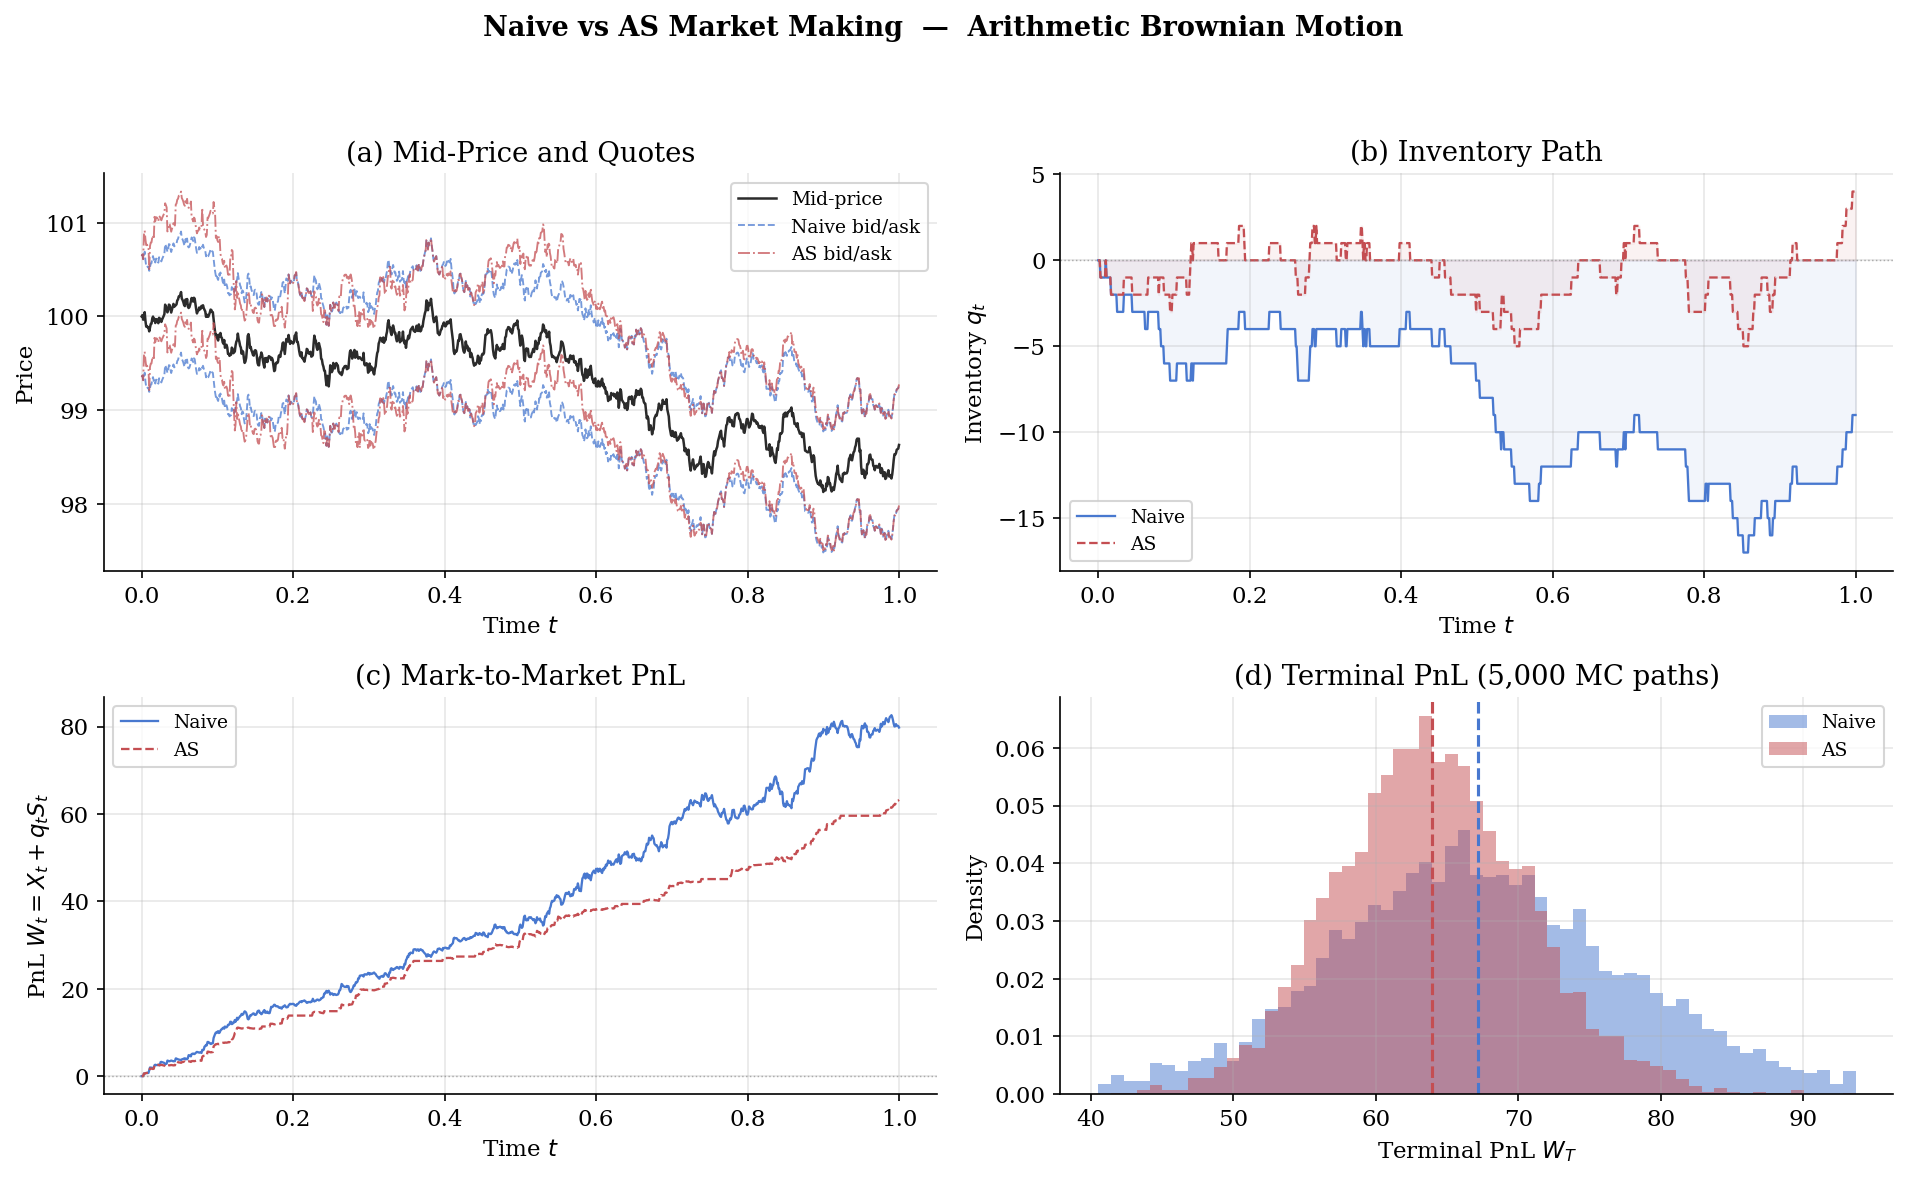
\includegraphics[width=0.85\textwidth]{1/py1.png}
\caption{Single-asset ABM comparison: naive versus Avellaneda--Stoikov quoting.}
\label{fig:bm_results}
\end{figure}

Figure~\ref{fig:bm_results} illustrates the ABM case. Panel (a) shows that both strategies quote around the same mid-price, but the AS quotes are not fixed symmetrically around $S_t$: they move with inventory through the reservation-price adjustment. When the dealer accumulates a long inventory, the quote center is pushed downward to make selling more likely and further buying less attractive; when the dealer is short, the opposite adjustment occurs. Panel (b) makes this mechanism visible. The naive inventory drifts much further from zero because the policy has no endogenous force pulling $q_t$ back toward neutrality, while the AS inventory is actively stabilized by the quote skew. Panel (c) should be read as a single realized path, not as the main performance criterion. In this particular path, the naive strategy ends higher because the realized price movement happens to reward the inventory exposure it has accumulated. Panel (d) is therefore the more relevant diagnostic: over $5{,}000$ paths, the naive terminal PnL distribution is wider, whereas the AS distribution is more concentrated. The message is that the AS rule does not simply try to maximize one lucky path; it reduces the dispersion generated by unmanaged inventory exposure.

\begin{figure}[H]
\centering
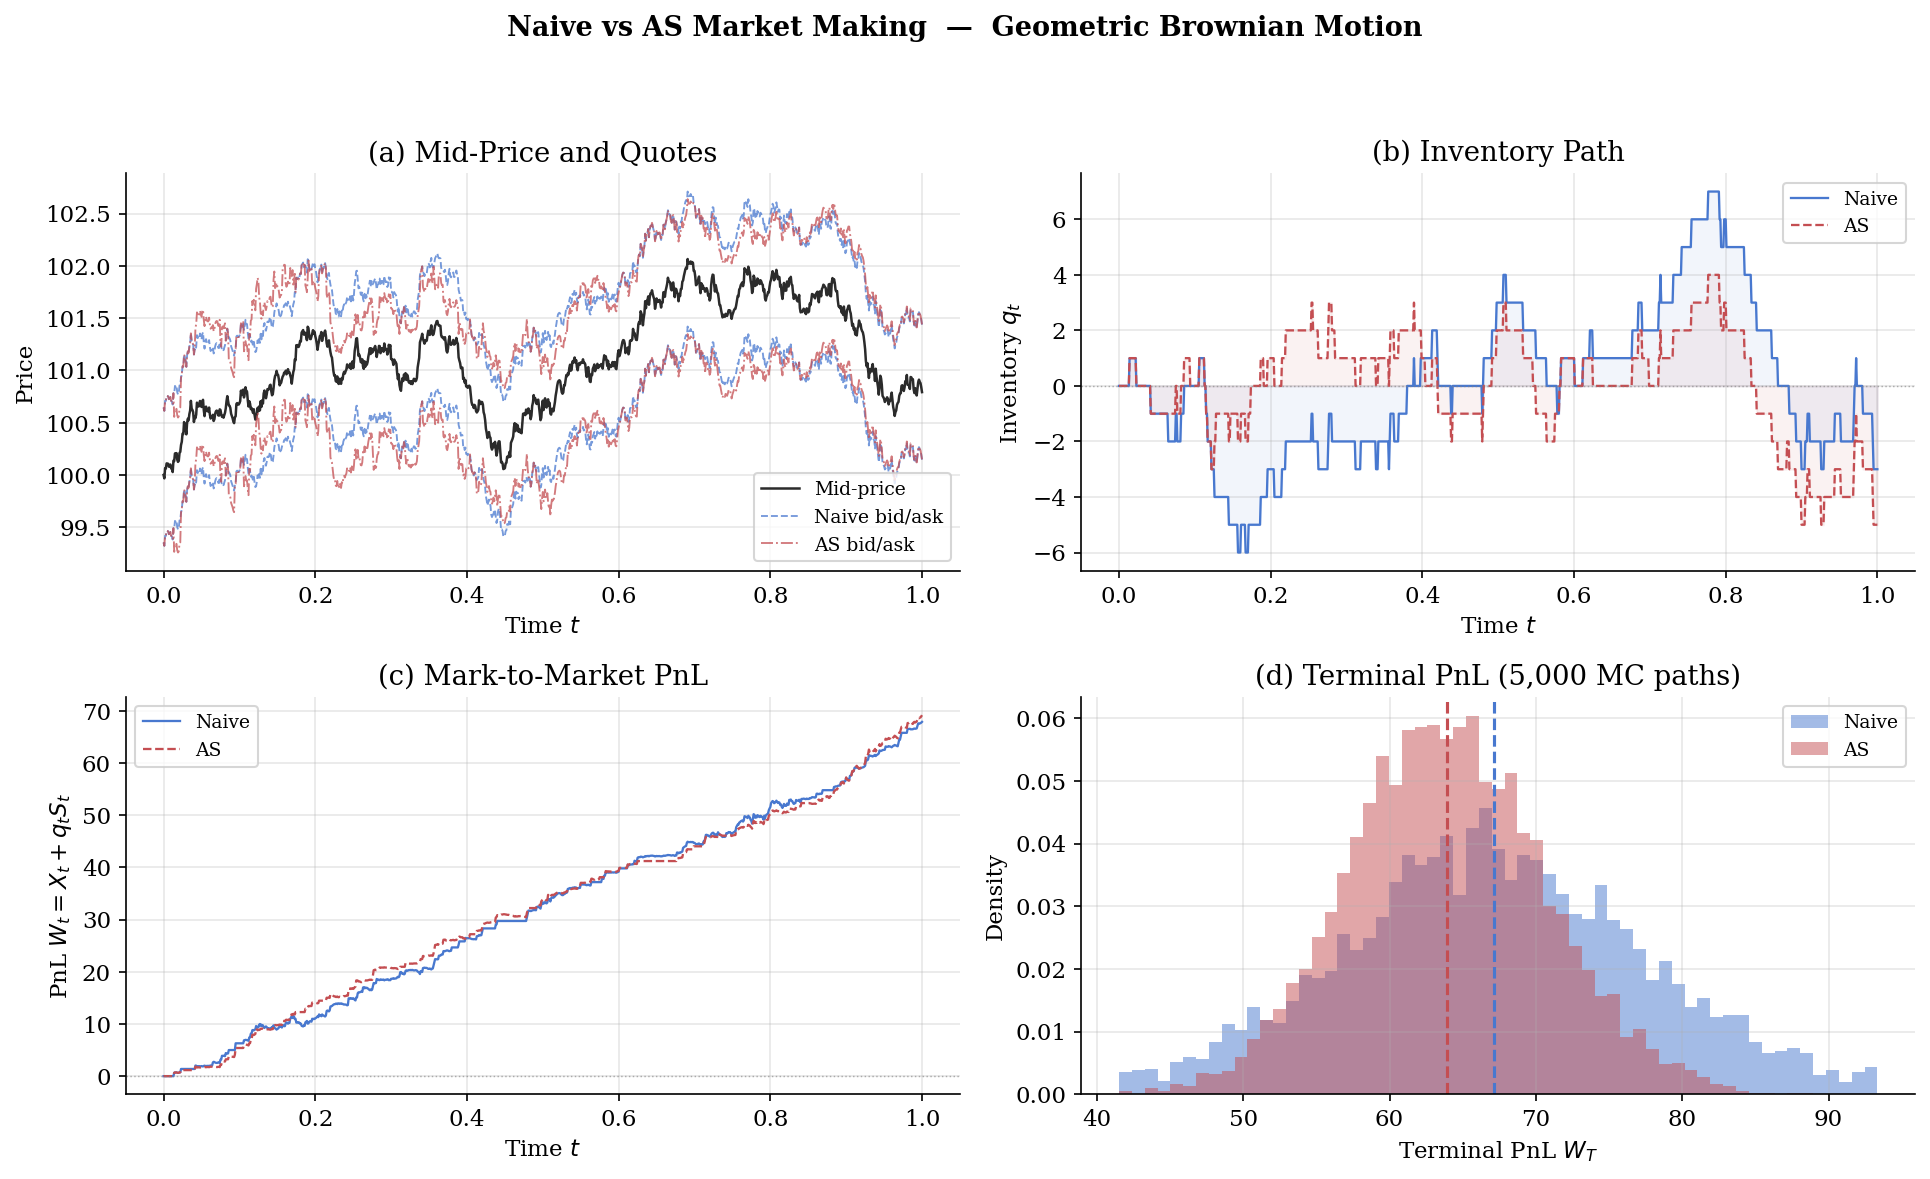
\includegraphics[width=0.85\textwidth]{1/py2.png}
\caption{Single-asset GBM comparison: naive versus Avellaneda--Stoikov quoting.}
\label{fig:gbm_results}
\end{figure}

Figure~\ref{fig:gbm_results} reports the GBM case. Since $\sigma_{GBM}S_0$ is calibrated to match the ABM dollar volatility, the aggregate Monte Carlo diagnostics are close to the ABM case. The difference is conceptual rather than cosmetic. Under GBM, the volatility parameter describes return risk, while the risk of holding one physical unit of inventory depends on the current price level. For this reason, the simulation uses the local monetary variance approximation $(\sigma_{GBM}S_t)^2$ inside the reservation price. When $S_t$ increases, one unit of inventory becomes riskier in dollar terms, and the AS quote skew reacts more strongly. This is why the GBM version is useful even if the numerical table is similar to ABM: it shows that inventory control should be expressed in monetary-risk units, not directly in return-volatility units.

\section{Covariance-Aware Multi-Asset Diagnostics}

The multivariate experiment uses three correlated arithmetic Brownian assets. Asset C is deliberately specified as inversely correlated with the first two assets, so that the covariance pressure $\Sigma q_t$ can differ sharply from the raw inventory vector $q_t$. This makes the key multi-asset mechanism visible: a position that looks large in physical units may be less dangerous if it hedges the rest of the book, while a small position may still be risky if it loads on the same covariance direction as the current portfolio.

\begin{figure}[H]
\centering
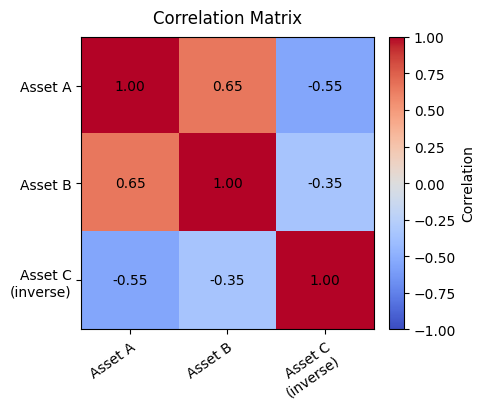
\includegraphics[width=0.58\textwidth]{img/1/Corr.png}
\caption{Correlation matrix used in the three-asset diagnostic. The matrix has unit diagonal entries, with $\rho_{AB}=0.65$, $\rho_{AC}=-0.55$, and $\rho_{BC}=-0.35$. Positive values indicate co-movement between assets, while negative values capture the inverse exposure of Asset C.}
\label{fig:correlation-matrix-three-asset}
\end{figure}

The corresponding covariance matrix $\Sigma$ combines these correlation coefficients with the individual asset volatilities. It is the matrix used by the covariance-aware policy to transform the raw inventory vector $q_t$ into the risk-pressure vector $\Sigma q_t$.

\begin{table}[H]
\centering
\small
\caption{Covariance matrix $\Sigma$ used in the three-asset diagnostic.}
\begin{tabular}{@{}lrrr@{}}
\toprule
 & Asset A & Asset B & Asset C (inverse) \\
\midrule
Asset A           &  2.2500 &  1.0725 & -0.7425 \\
Asset B           &  1.0725 &  1.2100 & -0.3465 \\
Asset C (inverse) & -0.7425 & -0.3465 &  0.8100 \\
\bottomrule
\end{tabular}
\end{table}

For $N=3{,}000$ Monte Carlo paths, the covariance-aware inventory policy again sacrifices a small amount of average PnL but materially improves the risk profile of the terminal book.

\begin{table}[H]
\centering
\small
\caption{Multivariate Monte Carlo diagnostics with $3{,}000$ simulated paths.}
\begin{tabularx}{\textwidth}{@{}Xrrr@{}}
\toprule
Metric & Naive & Inventory-based & Difference \\
\midrule
Mean terminal PnL                         & 158.709 & 154.556 & -4.153 \\
Std terminal PnL                          &  16.439 &  10.547 & -5.892 \\
Sharpe-like ratio                         &   9.654 &  14.654 &  5.000 \\
Mean $|$terminal inv$|$                   &  21.949 &  11.203 & -10.745 \\
Mean Std$(q_t)$                           &   6.593 &   3.397 & -3.195 \\
Mean turnover                             & 266.641 & 257.767 & -8.874 \\
Mean terminal risk $\|q_T\|_\Sigma$       &  17.051 &   7.419 & -9.632 \\
Median terminal risk $\|q_T\|_\Sigma$     &  15.313 &   6.996 & -8.318 \\
Mean average path risk                    &  11.397 &   3.925 & -7.472 \\
Mean max path risk                        &  22.638 &  10.065 & -12.573 \\
\bottomrule
\end{tabularx}
\end{table}

The multivariate results are stronger than the single-asset results because the naive policy is not merely ignoring inventory size; it is ignoring the entire covariance structure. The mean terminal risk norm $\|q_T\|_\Sigma=\sqrt{q_T^\top\Sigma q_T}$ falls from $17.051$ to $7.419$, while the mean maximum path risk falls from $22.638$ to $10.065$. The average gross terminal inventory also falls by more than ten units. These diagnostics show that covariance-aware control does not simply reduce each position mechanically; it reduces the risk of the portfolio after correlations are taken into account.

\begin{figure}[H]
\centering
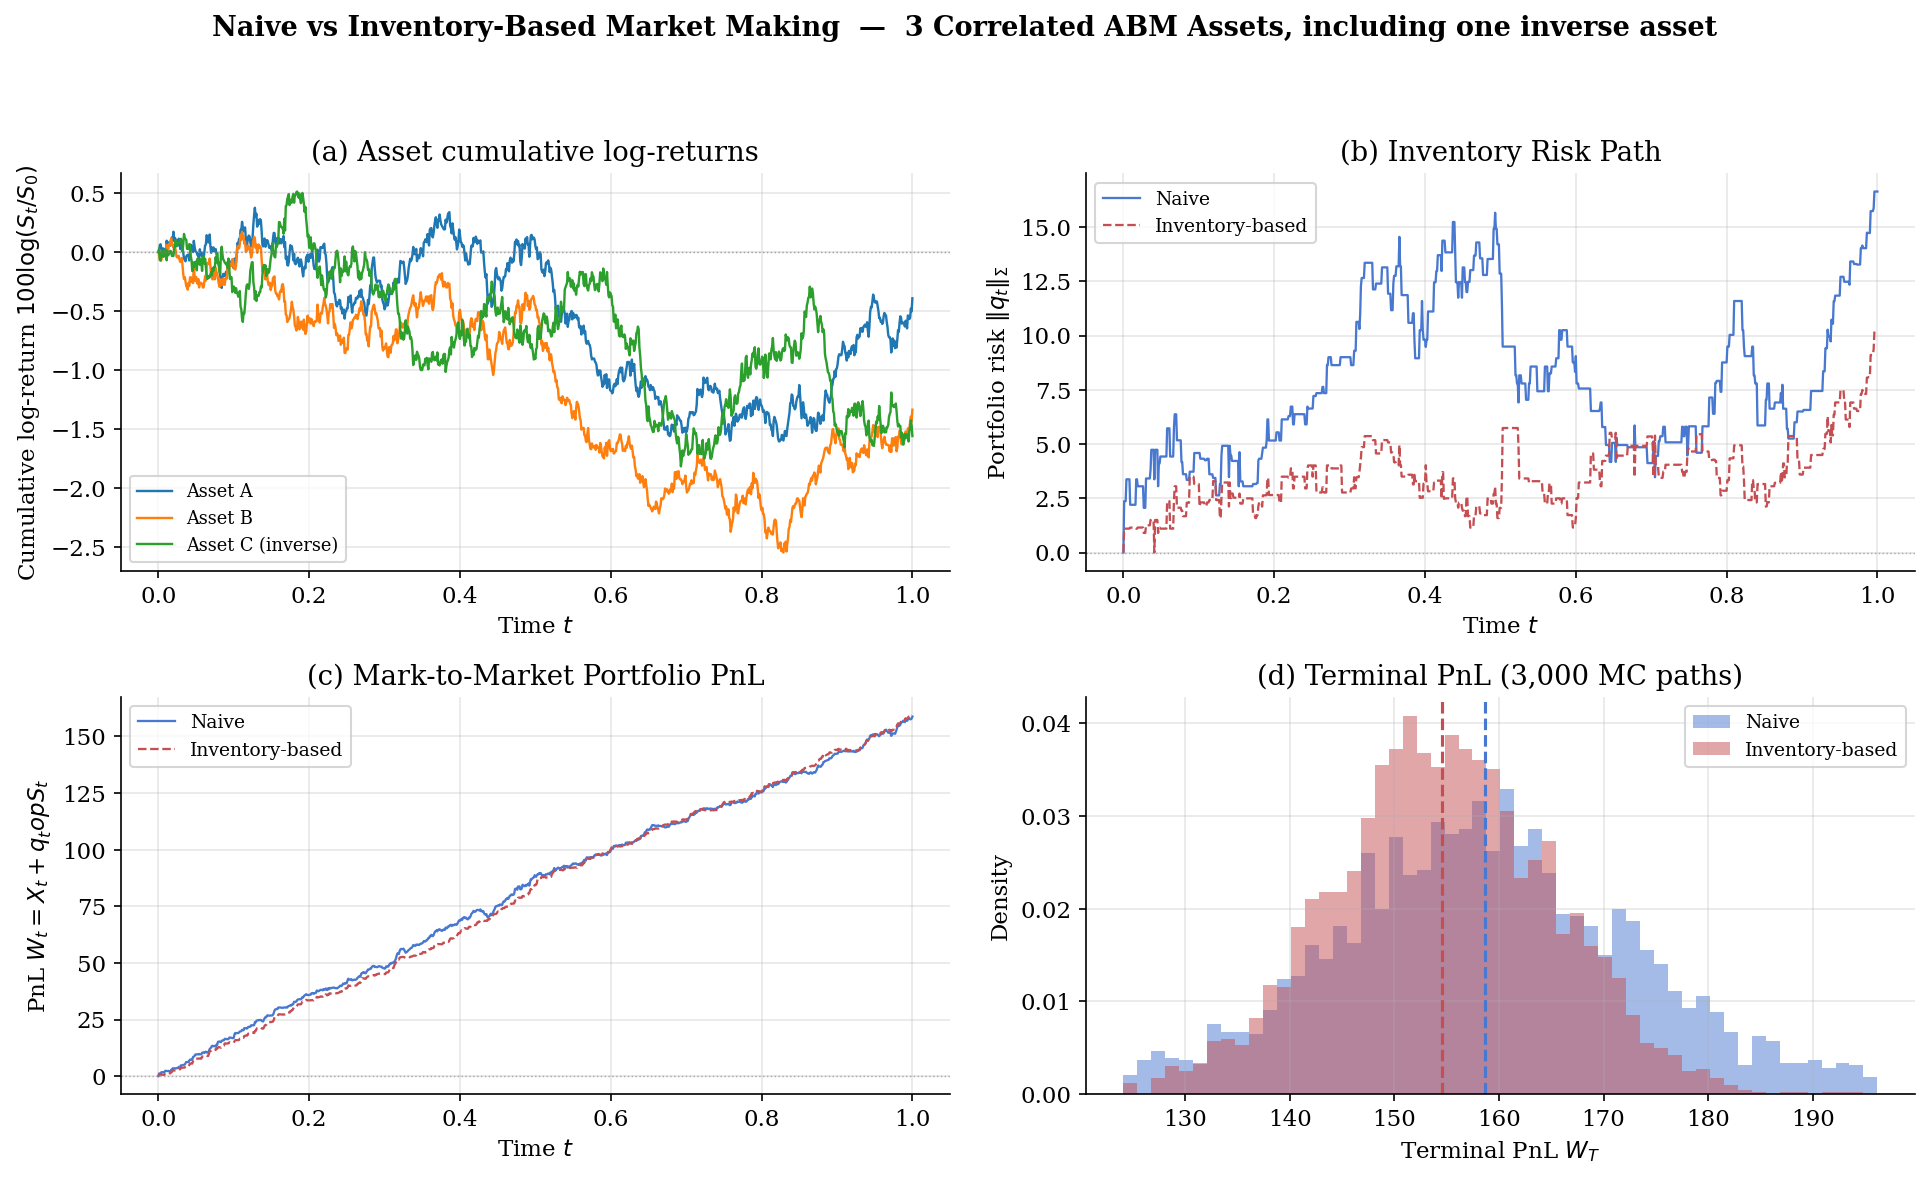
\includegraphics[width=0.96\textwidth]{1/py3.png}
\caption{Three-asset covariance-aware market-making diagnostic.}
\label{fig:multi_results}
\end{figure}

Figure~\ref{fig:multi_results} summarizes the three-asset diagnostic. Panel (a) reports cumulative log-returns, which makes the three price paths comparable even though the assets start from different price levels. The third asset is intentionally inversely correlated with the first two, so the relevant inventory signal is no longer the raw vector $q_t$ alone but the covariance-adjusted pressure $\Sigma q_t$. Panel (b) shows the portfolio risk norm $\|q_t\|_\Sigma$, which is the natural multivariate analogue of single-asset inventory risk. The naive strategy accumulates a much larger covariance-adjusted exposure because it treats each asset independently, while the inventory-based strategy keeps the risk path lower by reacting to the whole book. Panel (c) shows that both policies generate positive spread-capture PnL on the reference path, but the inventory-aware policy does so with a substantially lower portfolio-risk footprint. Panel (d) confirms the Monte Carlo result: the inventory-based terminal PnL distribution is more concentrated, while the naive policy leaves wider tails because it accepts larger covariance-adjusted inventory exposure. This is the key difference from the scalar case: the multi-asset dealer must control the risk of the book, not only the size of each single position.

Overall, the numerical evidence is consistent across all three experiments. The naive policy can look attractive if one only checks average PnL in a frictionless benchmark, but this comes from carrying more inventory risk. The Avellaneda--Stoikov policy is better understood as a risk-adjusted market-making rule: it reduces terminal inventory, lowers PnL volatility, and becomes especially valuable once the dealer manages a correlated book rather than a single isolated asset.

The conclusion collects these findings into the main methodological message of the article and clarifies how this benchmark can serve as the starting point for richer high-frequency market-making models.

\chapter*{Conclusion}
\addcontentsline{toc}{chapter}{Conclusion}
\markboth{Conclusion}{Conclusion}

This conclusion summarizes the benchmark contribution of the article. The paper develops the first benchmark layer of the project: the objective is not to reproduce the full complexity of real high-frequency markets, but to isolate the core mechanism of inventory-aware market making in a controlled setting. For this reason, the execution engine, accounting rules, fill probabilities, and Monte Carlo design are kept fixed across all experiments, while the mid-price model and the inventory state are progressively extended. The main message is that inventory-aware quoting reduces risk-adjusted exposure in both single-asset and covariance-aware settings, while leaving a clear baseline for future extensions with richer volatility and microstructure models.

The Avellaneda--Stoikov framework is useful because it formalizes the central trade-off of market making in a compact way: spread capture versus inventory and execution risk. In the single-asset setting, the arithmetic Brownian motion case provides the cleanest environment for interpreting the reservation price and the quote skew. The geometric Brownian motion case then shows why inventory risk should be measured in monetary terms: when volatility is proportional to the price level, the risk of holding one physical unit of inventory changes with the current price.

The simulation results are consistent with the expected risk-adjusted interpretation of the model. The naive symmetric strategy can sometimes display a slightly higher average terminal PnL in this simplified benchmark, because it accepts more inventory exposure and therefore captures spread without actively controlling the book. The inventory-based strategy, instead, materially reduces terminal inventory, intraday inventory variability, and terminal PnL dispersion. The improvement is especially visible in the Sharpe-like ratios and in the multivariate portfolio-risk diagnostics.

The covariance-aware extension clarifies the main conceptual message of the multi-asset setting. A dealer should not control each asset as an isolated single-name problem. Once assets are correlated, the relevant inventory signal is the contribution of each asset to the risk of the whole book. The quote of each asset must therefore react not only to its own inventory, but also to the way that asset co-moves with the rest of the portfolio. This is why the multivariate simulation reports both raw inventories and portfolio-risk diagnostics.

This first article should therefore be read as the classical baseline of the project. In future work, and in particular in the second article of the sequence, the same market-making logic can be tested under more complex price and volatility models. Natural extensions include stochastic volatility, volatility clustering, rough-volatility or Volterra-type specifications, jump components, state-dependent order flow, and richer microstructure mechanisms such as latency, queue priority, adverse selection, and market impact. These extensions will make the environment more realistic, but the benchmark developed here remains the reference point for understanding how each additional modelling layer changes the behaviour of the inventory-aware dealer.


\section*{Limitations}
\addcontentsline{toc}{section}{Limitations}

The benchmark is intentionally stylized. It should not be interpreted as a calibrated HFT backtest or as evidence that the reported PnL levels are attainable in a production environment. Its purpose is to isolate the mechanism of inventory-aware quoting under controlled assumptions.

Several important market features are deliberately excluded. The simulations use no historical market-data calibration, no explicit transaction fees, rebates, or exchange costs, no adverse-selection channel, no latency, no queue-position model, no market impact, no partial fills, and no endogenous order-flow response to the dealer's quotes. Fill probabilities are generated from a reduced-form intensity and then discretized over time steps.

The GBM case is treated through a local monetary-variance approximation, not as an exact closed-form solution of the GBM--CARA Avellaneda--Stoikov problem. Similarly, the multi-asset section should be read as a covariance-aware extension of the inventory-control logic, not as a complete high-dimensional HJB solution with all cross-asset microstructure effects. These restrictions make the benchmark transparent and reproducible, but they also define the boundary of the conclusions.

\begin{references}

\bibitem{AvellanedaStoikov2008}
Marco Avellaneda and Sasha Stoikov,
\emph{High-frequency trading in a limit order book},
\emph{Quantitative Finance} 8(3), 217--224, 2008.

\bibitem{BergaultEvangelistaGueantVieira2022}
Philippe Bergault, David Evangelista, Olivier Gu\'eant, and Douglas Vieira,
\emph{Closed-form approximations in multi-asset market making},
arXiv:1810.04383v5, 2022.

\bibitem{CarteaJaimungalPenalva2015}
\'Alvaro Cartea, Sebastian Jaimungal, and Jos\'e Penalva,
\emph{Algorithmic and High-Frequency Trading},
Cambridge University Press, 2015.

\bibitem{Glasserman2004}
Paul Glasserman,
\emph{Monte Carlo Methods in Financial Engineering},
Springer, 2004.

\bibitem{GouldEtAl2013}
Martin D. Gould, Mason A. Porter, Stuart Williams, Mark McDonald, Daniel J. Fenn, and Sam D. Howison,
\emph{Limit order books},
\emph{Quantitative Finance} 13(11), 1709--1742, 2013.

\bibitem{GueantLehalleFernandezTapia2013}
Olivier Gu\'eant, Charles-Albert Lehalle, and Joaquin Fernandez-Tapia,
\emph{Dealing with the inventory risk: a solution to the market making problem},
\emph{Mathematics and Financial Economics} 7(4), 477--507, 2013.

\bibitem{Gueant2016}
Olivier Gu\'eant,
\emph{The Financial Mathematics of Market Liquidity: From Optimal Execution to Market Making},
CRC Press, 2016.

\bibitem{Harris2003}
Larry Harris,
\emph{Trading and Exchanges: Market Microstructure for Practitioners},
Oxford University Press, 2003.

\bibitem{Hasbrouck2007}
Joel Hasbrouck,
\emph{Empirical Market Microstructure: The Institutions, Economics, and Econometrics of Securities Trading},
Oxford University Press, 2007.

\bibitem{OHara1995}
Maureen O'Hara,
\emph{Market Microstructure Theory},
Blackwell, 1995.

\bibitem{RostagnoFlorio2026MonteCarlo}
Andrea Rostagno and Francesco Florio,
\emph{Monte Carlo Methods and Portfolio Simulation: Theory, Convergence, and Applications to Risk Analysis},
Starting Finance Club PoliTo Research Area, 2026.
Reviewed by Salvatore Messina.
\bibitem{githubrepo}
S. G. Messina and N. Soriano,
\emph{High-Frequency Market Making under Avellaneda--Stoikov: Classical Diffusions and Multi-Asset Inventory Control: supporting code},
Starting Finance Club PoliTo, GitHub repository,
\url{https://github.com/StartingFinanceClubPoliTo/Research/tree/51d8ecb67452fd5bb428253fcee6cf3001884f63/Stoikov-Avellonada/Article-1},
accessed 15/05/2026.
\end{references}
\end{document}
